% \documentclass[../main-physics-workbook.tex]{subfiles}
\documentclass[]{exam}
\usepackage{marvosym}

%...TikZ & PGF
\usepackage{pgfplots}
\pgfplotsset{compat=1.11}
\tikzset{>=latex}
\usetikzlibrary{calc,math}
\usepackage{tikzsymbols}
\usepgfplotslibrary{fillbetween}
\usetikzlibrary{decorations.markings} 
\usetikzlibrary{arrows.meta} %...APP2 for arrows as objects and images
\usetikzlibrary{backgrounds} %...For shading portions of graphs
\usetikzlibrary{patterns} %...Unit 5 Problems
\usetikzlibrary{shapes.geometric} %...For drawing cylinders in Unit 2
\usepackage{makecell} %...use \thead{} to enable line skip in table headers
\tikzset{
    mark position/.style args={#1(#2)}{
        postaction={
            decorate,
            decoration={
                markings,
                mark=at position #1 with \coordinate (#2);
            }
        }
    }
} %...See https://tex.stackexchange.com/questions/43960/define-node-at-relative-coordinates-of-draw-plot

\tikzset{
    declare function = {trajectoryequation10(\x,\vi,\thetai)= tan(\thetai)*\x - 10*\x^2/(2*(\vi*cos(\thetai))^2);},
    declare function = {trajectoryequation(\x,\vi,\thetai)= tan(\thetai)*\x - 9.8*\x^2/(2*(\vi*cos(\thetai))^2);},
    declare function = {patheq(\x,\yi,\vi,\thetai)= \yi + tan(\thetai)*\x - 9.8*\x^2/(2*(\vi*cos(\thetai))^2);},
    declare function = {patheqten(\x,\yi,\vi,\thetai)= \yi + tan(\thetai)*\x - 10*\x^2/(2*(\vi*cos(\thetai))^2);} %like patheq but with gravity = 10
}

%...siunitx
\usepackage{siunitx}
\DeclareSIUnit{\nothing}{\relax}
\def\mymu{\SI{}{\micro\nothing} }
\DeclareSIUnit\mmHg{mmHg}
\DeclareSIUnit{\mile}{mi}
%...NOTE: "The product symbol between the number and unit is set using the quantity-product option."

%...Other
\usepackage{amsthm}
\usepackage{amsmath}
\usepackage{amssymb}
\usepackage{cancel}
\usepackage{subcaption}
\usepackage{dashrule}
\usepackage{enumitem}
\usepackage{fontawesome}
\usepackage{multicol}
\usepackage{glossaries}
%\numberwithin{equation}{section}
\numberwithin{figure}{section}
\usepackage{float}
\usepackage{twemojis} %...twitter emojis
\usepackage{utfsym}
\usepackage{linearb} %...For \BPwheel in Unit 8
\newcommand{\R}{\mathbb{R}} %...real number symbol
\usepackage{graphicx}
\graphicspath{ {../Figures/} }
\usepackage{hyperref}
\hypersetup{colorlinks=true,
    linkcolor=blue,
    filecolor=magenta,
    urlcolor=cyan,}
\urlstyle{same}
\newcommand{\hdashline}{{\hdashrule{\textwidth}{0.5pt}{0.8mm}}}
\newcommand{\hgraydashline}{{\color{lightgray} \hdashrule{0.99\textwidth}{1pt}{0.8mm}}}

%...Miscellaneous user-defined symbols
\newcommand{\fnet}{F_{\text{net}}} %...For net force
\newcommand{\bvec}[1]{\vec{\mathbf{#1}}} %...bold vector
\newcommand{\bhat}[1]{\,\hat{\mathbf{#1}}} %...bold hat vector
\newcommand{\que}{\mathord{?}}  %...Question mark symbol in equation env
%...Define thick horizontal rule for examples:
\newcommand{\hhrule}{\hrule\hrule}
\let\oldtexttt\texttt% Store \texttt
\renewcommand{\texttt}[2][black]{\textcolor{#1}{\ttfamily #2}}% 

%...For use in the exam document class
\newif\ifprintmetasolutions


%...Decreases space above and below align and gather enironment
\makeatletter
\g@addto@macro\normalsize{%
  \setlength\abovedisplayskip{-3pt}
  \setlength\belowdisplayskip{6pt} 
}
\makeatother





\usepackage[margin=1in]{geometry}
\usepackage[figurewithin=none]{caption}
\usepackage{exam-randomizechoices}
\setrandomizerseed{1}

\CorrectChoiceEmphasis{\color{red}\bfseries}
\renewcommand{\solutiontitle}{\noindent\textbf{\textcolor{red}{Solution:}}\enspace}

\usepackage{OutilsGeomTikz}
\usepackage{utfsym} %...Symbols in Unit 7 Problems
\usepackage{tabu} %...Symbols in Unit 7 Problems

%...For use in Unit 2            %    
\setlength{\columnsep}{2cm}      %
\setlength{\columnseprule}{1pt}  %
\usepackage[none]{hyphenat}      %
%%%%%%%%%%%%%%%%%%%%%%%%%%%%%%%%%

%...For use in Unit 11 on Waves:
\pgfdeclarehorizontalshading{visiblelight}{50bp}{  %
color(0.00000000000000bp)=(red);                   %
color(8.33333333333333bp)=(orange);                %
color(16.66666666666670bp)=(yellow);               %
color(25.00000000000000bp)=(green);                %
color(33.33333333333330bp)=(cyan);                 %
color(41.66666666666670bp)=(blue);                 %
color(50.00000000000000bp)=(violet)                %
}                                                  %

\newcommand{\checkbox}[1]{%
  \ifnum#1=1
    \makebox[0pt][l]{\raisebox{0.15ex}{\hspace{0.1em}\Large$\checkmark$}}%
  \fi
  $\square$%
}
%%%%%%%%%%%%%%%%%%%%%%%%%%%%%%%%%%%%%%%%%%%%%%%%%%%%

%...If using circuitikz package:
% \ctikzset{bipoles/battery1/height=0.5}
% \ctikzset{bipoles/battery1/width=0.25}
% \ctikzset{bipoles/resistor/height=0.15}
% \ctikzset{bipoles/resistor/width=0.4}
\makenoidxglossaries

%...UNIT 1: CONSTANT MOTION

\newglossaryentry{scalar}{
    name=scalar,
    description={a quantity that has magnitude (and possibly sign) but no direction}
}

\newglossaryentry{magnitude}{
    name={magnitude},
    description={size or amount}
}

\newglossaryentry{vector}{
    name={vector},
    description={a quantity that has both magnitude and direction}
}

\newglossaryentry{tail}{
    name={tail},
    description={the starting point of a vector; the point opposite to the head or tip of the arrow}
}

\newglossaryentry{head}{
    name={head},
    description={the end point of a vector; the location of the vector's arrow; also referred to as the tip}
}

\newglossaryentry{head-to-tail method}{
    name={head-to-tail method},
    description={a method of adding vectors in which the tail of each vector is placed at the head of the previous vector}
}

\newglossaryentry{position}{
    name={position},
    description={the location of an object at any particular time}
}

\newglossaryentry{reference frame}{
    name={reference frame},
    description={a coordinate system from which the positions of objects are described}
}


\newglossaryentry{displacement}{
    name={displacement},
    description={the change in position of an object against a fixed axis}
}

\newglossaryentry{distance}{
    name={distance},
    description={the length of the path actually traveled between an initial and a final position}
}

\newglossaryentry{position vs. time graph}{
    name={position vs. time graph},
    description={a graph in which position is plotted on the vertical axis and time is plotted on the horizontal axis}
}

\newglossaryentry{speed}{
    name={speed},
    description={rate at which an object changes its location}
}

\newglossaryentry{average speed}{
    name={average speed},
    description={distance traveled divided by the time during which the motion occurs}
}

\newglossaryentry{velocity}{
    name={velocity},
    description={the speed and direction of an object}
}

\newglossaryentry{average velocity}{
    name={average velocity},
    description={displacement divided by the time during which the displacement occurs}
}

\newglossaryentry{velocity vs. time graph}{
    name={velocity vs. time graph},
    description={a graph in which velocity is plotted on the vertical axis and time is plotted on the horizontal axis}
}

\newglossaryentry{mass}{
    name=mass,
    description={the quantity of matter in a substance; the SI unit of mass is the kilogram}
}

\newglossaryentry{inertia}{
    name=inertia,
    description={the tendency of an object at rest to remain at rest, or for a moving object to remain in motion in a straight line and at a constant speed}
}

\newglossaryentry{Newton's first law of motion}{
    name={Newton's first law of motion},
    description={a body at rest remains at rest or, if in motion, remains in motion at a constant speed in a straight line, unless acted on by a net external force; also known as the law of inertia}
}

\newglossaryentry{momentum}{
    name={momentum},
    description={the product of a system's mass and velocity}
}

\newglossaryentry{momentum vs. time graph}{
    name={momentum vs. time graph},
    description={a graph in which momentum is plotted on the vertical axis and time is plotted on the horizontal axis}
}

\newglossaryentry{kinetic energy}{
    name={kinetic energy},
    description={energy of motion}
}

\newglossaryentry{joule}{
    name=joule,
    description={the metric unit for work and energy; equal to 1 newton meter ($\text{N}\cdot\text{m}$)}
}

\newglossaryentry{relative speed}{
    name={relative speed},
    description={how fast or slow an object appears to be moving to another object}
}

\newglossaryentry{relative velocity}{
    name={relative velocity},
    description={the rate at which an object changes position relative to another object}
}

%...UNIT 2: FORCE INTERACTIONS

\newglossaryentry{force}{
    name=force,
    description={a push or pull on an object with a specific magnitude and direction; can be represented by vectors; can be expressed as a multiple of a standard force; the SI unit of force is the Newton (N)}
}

\newglossaryentry{external force}{
    name=external force,
    description={a force acting on an object or system that originates outside of the object or system}
}

\newglossaryentry{free body diagram}{
    name=free body diagram,
    description={a diagram showing all external forces acting on a body}
}

\newglossaryentry{frictional force}{
    name=frictional force,
    description={an external force that acts opposite to the direction of motion or, for when there is no relative motion, in the direction needed to prevent slipping}
}

\newglossaryentry{applied force}{
    name={applied force},
    description={a contact force intentionally implied by a person on an object}
}


\newglossaryentry{gravitational force}{
    name=gravitational force, %...MY DEFINITION
    description={the downward force on an object due to the attraction by the Earth or other massive body}
}

\newglossaryentry{net force}{
    name=net force,
    description={the sum of all forces acting on an object or system}
}

\newglossaryentry{normal force}{
    name=normal force,
    description={that component of the contact force between two objects, which acts perpendicularly to and away from their plane of contact}
}

\newglossaryentry{tension}{
    name=tension,
    description={a pulling force that acts along a connecting medium, especially a stretched flexible connector, such as a rope or cable; when a rope supports the weight of an object, the force exerted on the object by the rope is called tension}
}

\newglossaryentry{spring force}{
    name=spring force, %...From district slides
    description={a force applied from a spring when it is either compressed or stretched}
}

%...UNIT 3: ACCELERATION

\newglossaryentry{acceleration}{
    name={acceleration},
    description={a change in velocity over time}
}

\newglossaryentry{average acceleration}{
    name={average acceleration},
    description={change in velocity divided by the time interval over which it changed}
}

%...UNIT 4:


\newglossaryentry{impulse}{
    name={impulse},
    description={average net external force multiplied by the time the force acts; equal to the change in momentum}
}

\newglossaryentry{impulse-momentum theorem}{
    name={impulse-momentum theorem},
    description={the impulse equals change in momentum}
}

\newglossaryentry{work}{
    name={work},
    description={force multiplied by distance}
}

%...UNIT 5: FORCE ANALYSIS

\newglossaryentry{Newton's universal law of gravitation}{
    name={Newton's universal law of gravitation},
    description={states that gravitational force between two objects is directly proportional to the product of their masses and inversely proportional to the square of the distance between them}
}

\newglossaryentry{gravitational constant}{
    name={gravitational constant},
    description={the proportionality constant in Newton's law of universal gravitation}
}

\newglossaryentry{weight}{
    name={weight},
    description={the force of gravity, $W$, acting on an object of mass $m$; defined mathematically as $W = mg$, where $g$ is the acceleration due to gravity}
}

\newglossaryentry{contact force}{
    name={contact force},
    description={a type of force that occurs when objects are physically in contact with each other}
}

%...UNIT 6: ONE-DIMENSIONAL MOTION

\newglossaryentry{free fall}{
    name=free fall,
    description={a situation in which the only force acting on an object is the force of gravity}
}

\newglossaryentry{kinematic equations}{
    name={kinematic equations},
    description={the 
    %five 
    equations that describe constant acceleration motion in terms of time, displacement, velocity, and acceleration}
}

%...UNIT 7: MOTION IN TWO DIMENSIONS

\newglossaryentry{projectile}{
    name={projectile},
    description={an object that travels through the air and experiences only acceleration due to gravity}
}

\newglossaryentry{projectile motion}{
    name={projectile motion},
    description={the motion of an object that is subject only to the acceleration of gravity}
}

\newglossaryentry{trajectory}{
    name={trajectory},
    description={the path of a projectile through the air}
}

\newglossaryentry{apex}{
    name={apex},
    description={the location on the trajectory at which the projectile reaches maximum height}
}

\newglossaryentry{hang time}{
    name={hang time},
    description={the amount of time that a projectile is in the air during projectile motion}
}

\newglossaryentry{horizontally launched projectile}{
    name={horizontally launched projectile},
    description={a projectile whose initial velocity is entirely in the horizontal direction}
}

\newglossaryentry{impact speed}{
    name={impact speed},
    description={the speed at which a projectile strikes the ground after being launched}
}

%...UNIT 8: CONSERVATION IN MECHANICAL SYSTEMS

\newglossaryentry{system}{
    name={system},
    description={one or more objects of interest for which only the forces acting on them from the outside are considered, but not the forces acting between them or inside them}
}

\newglossaryentry{energy}{
    name={energy},
    description={the ability to do work}
}

\newglossaryentry{potential energy}{
    name={potential energy},
    description={stored energy}
}

\newglossaryentry{gravitational potential energy}{
    name={gravitational potential energy},
    description={energy acquired by doing work against gravity}
}

\newglossaryentry{law of conservation of energy}{
    name={law of conservation of energy},
    description={states that energy is neither created nor destroyed}
}

\newglossaryentry{mechanical energy}{
    name={mechanical energy},
    description={kinetic plus potential energy}
}

\newglossaryentry{elastic collision}{
    name={elastic collision},
    description={a collision in which objects separate after impact and kinetic energy is conserved}
}

\newglossaryentry{inelastic collision}{
    name={inelastic collision},
    description={a collision in which kinetic energy is not conserved}
}

\newglossaryentry{isolated system}{
    name={isolated system},
    description={system in which the net external force is zero}
}

\newglossaryentry{law of conservation of momentum}{
    name={law of conservation of momentum},
    description={when the net external force is zero, the total momentum of the system is conserved or constant}
}

\newglossaryentry{perfectly inelastic collision}{
    name={perfectly inelastic collision},
    description={collision in which objects stick together after impact and kinetic energy is not conserved}
}

\newglossaryentry{recoil}{
    name={recoil},
    description={backward movement of an object caused by the transfer of momentum from another object in a collision}
}

%...UNIT 9: CONSERVATION OF CHARGE

\newglossaryentry{electric charge}{
    name={electric charge},
    description={a physical property of an object that causes it to be attracted toward or repelled from another charged object; each charged object generates and is influenced by a force called an electromagnetic force}
}

\newglossaryentry{elementary charge}{
    name={elementary charge},
    description={the smallest observed unit of charge that can be isolated in nature; also, the magnitude of charge on 1 proton or 1 electron}
}

\newglossaryentry{electron}{
    name={electron},
    description={subatomic particle that carries one indivisible unit of negative electric charge}
}

\newglossaryentry{proton}{
    name={proton},
    description={subatomic particle that carries the same magnitude charge as the electron, but its charge is positive}
}

\newglossaryentry{electric field}{
    name={electric field},
    description={defines the force per unit charge at all locations in space around a charge distribution}
}

\newglossaryentry{law of conservation of charge}{
    name={law of conservation of charge},
    description={states that total charge is constant in any process}
}

\newglossaryentry{polarization}{
    name={polarization},
    description={separation of charge induced by nearby excess charge}
}

\newglossaryentry{Coulomb's law}{
    name={Coulomb's law},
    description={describes the electrostatic force between charged objects, which is proportional to the charge on each object and inversely proportional to the square of the distance between the objects}
}

\newglossaryentry{electric circuit}{
    name={electric circuit},
    description={physical network of paths through which electric current can flow}
}

\newglossaryentry{simple circuit}{
    name={simple circuit},
    description={a circuit with a single voltage source and a single resistor}
}

\newglossaryentry{electric current}{
    name={electric current},
    description={electric charge that is moving}
}


\newglossaryentry{Ohm's law}{
    name={Ohm's law},
    description={electric current is proportional to the voltage applied across a circuit or other path}
}

\newglossaryentry{resistance}{
    name={resistance},
    description={how much a circuit element opposes the passage of electric current; it appears as the constant of proportionality in Ohm’s law}
}

\newglossaryentry{resistor}{
    name={resistor},
    description={circuit element that provides a known resistance}
}

% \newglossaryentry{potential difference (or voltage)}{
%     name={potential difference (or voltage)},
%     description={change in potential energy of a charge moved from one point to another, divided by the charge; units of potential difference are joules per coulomb, known as volt}
% }

\newglossaryentry{voltage}{
    name={voltage},
    description={the electrical potential energy per unit charge; electric pressure created by a power source, such as a battery}
}

\newglossaryentry{electric power}{
    name={electric power},
    description={rate at which electric energy is transferred in a circuit}
}

\newglossaryentry{equivalent resistor}{
    name={equivalent resistor},
    description={resistance of a single resistor that is the same as the combined resistance of a group of resistors}
}

\newglossaryentry{in series}{
    name={in series},
    description={when elements in a circuit are connected one after the other in the same branch of the circuit}
}

\newglossaryentry{in parallel}{
    name={in parallel},
    description={when a group of resistors are connected side by side, with the top ends of the resistors connected together by a wire and the bottom ends connected together by a different wire}
}

\newglossaryentry{induction}{
    name={induction},
    description={creating an unbalanced charge distribution in an object by moving a charged object toward it (but without touching)}
}

%...UNIT 10: ELECTROMAGNETIC INDUCTION

\newglossaryentry{magnetic dipole}{
    name={magnetic dipole},
    description={term that describes magnets because they always have two poles: north and south}
}

\newglossaryentry{magnetic field}{
    name={magnetic field},
    description={directional lines around a magnetic material that indicates the direction and magnitude of the magnetic force}
}

\newglossaryentry{magnetic pole}{
    name={magnetic pole},
    description={part of a magnet that exerts the strongest force on other magnets or magnetic material}
}

\newglossaryentry{electromagnetic induction}{
    name={electromagnetic induction},
    description={rate at which energy is drawn from a source per unit current flowing through a circuit}
}


\newglossaryentry{Faraday's law}{
    name={Faraday's law},
    description={the means of calculating the emf in a coil due to changing magnetic flux}
}

\newglossaryentry{electromagnet}{
    name={electromagnet},
    description={device that uses electric current to make a magnetic field}
}

\newglossaryentry{transformer}{
    name={transformer},
    description={device that transforms voltages from one value to another}
}

\newglossaryentry{electric motor}{
    name={electric motor},
    description={device that transforms electrical energy into mechanical energy}
}

\newglossaryentry{generator}{
    name={generator},
    description={device that transforms mechanical energy into electrical energy}
}

%...UNIT 11: SIMPLE HARMONIC MOTION & WAVES

\newglossaryentry{wave}{
    name={wave},
    description={a disturbance that moves from its source and carries energy}
}

\newglossaryentry{wave velocity}{
    name={wave velocity},
    description={speed at which the disturbance moves; also called the propagation velocity or propagation speed}
}

\newglossaryentry{wavelength}{
    name={wavelength},
    description={distance between adjacent identical parts of a wave}
}

\newglossaryentry{wave cycle}{
    name={wave cycle},
    description={any portion of a wave encompassed by 1 wavelength}
}

\newglossaryentry{transverse wave}{
    name={transverse wave},
    description={a wave in which the disturbance is perpendicular to the direction of propagation}
}

\newglossaryentry{medium}{
    name={medium},
    description={the solid, liquid, or gas material through which a wave propagates}
}

\newglossaryentry{mechanical wave}{
    name={mechanical wave},
    description={wave that requires a medium through which it can travel}
}

\newglossaryentry{longitudinal wave}{
    name={longitudinal wave},
    description={wave in which the disturbance is parallel to the direction of propagation}
}

\newglossaryentry{constructive interference}{
    name={constructive interference},
    description={when two waves arrive at the same point exactly in phase; that is, the crests of the two waves are precisely aligned, as are the troughs}
}

\newglossaryentry{destructive interference}{
    name={destructive interference},
    description={when two identical waves arrive at the same point exactly out of phase that is precisely aligned crest to trough}
}

\newglossaryentry{oscillate}{
    name={oscillate},
    description={to move back and forth regularly between two points}
}

\newglossaryentry{amplitude}{
    name={amplitude},
    description={the maximum displacement from the equilibrium position of an object oscillating around the equilibrium position}
}

\newglossaryentry{frequency}{
    name={frequency},
    description={number of wave cycles per unit of time}
}

\newglossaryentry{simple harmonic motion}{
    name={simple harmonic motion},
    description={the oscillatory motion in a system where the net force can be described by Hooke’s law}
}

\newglossaryentry{simple harmonic oscillator}{
    name={simple harmonic oscillator},
    description={a device that oscillates in SHM,  such as a mass that is attached to a spring, where the restoring force is proportional to the displacement and acts in the direction opposite to the displacement}
}

\newglossaryentry{period}{
    name={period},
    description={the time it takes to complete one oscillation}
}

\newglossaryentry{electromagnetic wave}{
    name={electromagnetic wave},
    description={a radiant energy wave that consists of oscillating electric and magnetic fields}
}

\newglossaryentry{electromagnetic radiation}{
    name={electromagnetic radiation},
    description={radiant energy that consists of oscillating electric and magnetic fields}
}









%... Overview and Student Learning Expectations (OSLE)

\newglossaryentry{OSLE 6.1.a}{
    name={OSLE 6.1.a},
    description={compare the gravitational field strength on Earth to the acceleration due to gravity on Earth}
}

\newglossaryentry{OSLE 6.1.b}{
    name={OSLE 6.1.b},
    description={explain using universal gravitation and $F_\mathrm{net}=ma$ why all objects near Earth's surface fall at the same rate when in free fall}
}

\newglossaryentry{OSLE 6.1.c}{
    name={OSLE 6.1.c},
    description={explain the relationship between the mass, initial position, and initial velocity of an object in free fall on its final velocity and/or time in free fall}
}

\newglossaryentry{OSLE 6.1.d}{
    name={OSLE 6.1.d},
    description={describe the displacement, velocity, momentum, kinetic energy, and acceleration of an object in free fall that was dropped, thrown upward, or thrown downward using Multiple Representations}
}

\newglossaryentry{OSLE 6.1.e}{
    name={OSLE 6.1.e},
    description={relate the gravitational force, impulse, and work done on the object by the Earth to the object's change in velocity (acceleration), momentum, and kinetic energy}
}

        
\newglossaryentry{OSLE 6.2.a}{
    name={OSLE 6.2.a},
    description={describe what is known about an object's motion in a constant acceleration word problem using Multiple Representations}
}

\newglossaryentry{OSLE 6.2.b}{
    name={OSLE 6.2.b},
    description={solve for various unknown quantities utilizing kinematic equations when data is given in Multiple Representations for objects moving horizontally with constant acceleration}
}

\newglossaryentry{OSLE 6.3.c}{
    name={OSLE 6.3.c},
    description={solve for various unknown quantities utilizing kinematic equations when data is given in Multiple Representations for objects moving vertically with constant acceleration (free fall)}
}

\newglossaryentry{OSLE 6.4.d}{
    name={OSLE 6.4.d},
    description={solve multi-step problems that connect kinematic equations, the Law of Acceleration, Work-Energy Theorem, and/or the Impulse-Momentum Theorem}
}

\newglossaryentry{OSLE 7.1.a}{
    name={OSLE 7.1.a},
    description={compare the trajectory, hang time, max height, range, and final velocity of various projectiles that have different initial velocities, launch heights, launch angles, and masses, only varying one parameter at a time}
}

\newglossaryentry{OSLE 7.1.b}{
    name={OSLE 7.1.b},
    description={identify if and explain how the  initial velocity, launch height, launch angle, and mass of a projectile influence its motion---hang time, height, range, final velocity}
}

\newglossaryentry{OSLE 7.2.a}{
    name={OSLE 7.2.a},
    description={describe the vertical and horizontal motion of a projectile with a launch angle of zero using Multiple Representations}
}

\newglossaryentry{OSLE 7.2.b}{
    name={OSLE 7.2.b},
    description={illustrate the resultant motion of the projectile at any point in its trajectory as well as the relationship between the horizontal and vertical components using vector addition}
}

\newglossaryentry{OSLE 7.2.c}{
    name={OSLE 7.2.c},
    description={analyze and solve word problems about the motion of  horizontally launched projectiles using kinematic equations, vector addition, and  Multiple Representations}
}

\newglossaryentry{OSLE 7.3.a}{
    name={OSLE 7.3.a},
    description={describe the motion of an object moving with uniform circular motion in terms of centripetal force, centripetal acceleration, momentum, kinetic energy, and tangential velocity using Multiple Representations}
}

\newglossaryentry{OSLE 7.3.b}{
    name={OSLE 7.3.b},
    description={determine the centripetal force, mass, centripetal acceleration, tangential velocity, or radius of an object in circular motion}
}

\newglossaryentry{OSLE 7.4.a}{
    name={OSLE 7.4.a},
    description={predict the effects of changing the radius or mass of objects in orbiting systems using concepts of uniform circular motion and Newton’s law of universal gravitation}
}


\newglossaryentry{OSLE 8.1.a}{
    name={OSLE 8.1.a},
    description={identify multiple choices for a system given a scenario}
}

\newglossaryentry{OSLE 8.1.b}{
    name={OSLE 8.1.b},
    description={recognize that energy can be stored in the arrangement of particles or objects in a system as potential energy}
}

\newglossaryentry{OSLE 8.1.c}{
    name={OSLE 8.1.c},
    description={identify and calculate (i) gravitational potential energy and (ii) elastic potential energy when a system includes energy stored in the arrangement of its particles or objects}
}

\newglossaryentry{OSLE 8.1.d}{
    name={OSLE 8.1.d},
    description={compare the potential energy of a scenario for various choices of system}
}

\newglossaryentry{OSLE 8.1.e}{
    name={OSLE 8.1.e},
    description={identify, represent using multiple representations, and calculate the total mechanical energy present in a physical system}
}

\newglossaryentry{OSLE 8.1.f}{
    name={OSLE 8.1.f},
    description={predict the effects of changing the mass, velocity, height, gravitational field strength, spring constant, compression or stretching distance on the amount of $E_k$, $E_\mathrm{GP}$, and $E_\mathrm{SP}$}
}

\newglossaryentry{OSLE 8.1.g}{
    name={OSLE 8.1.g},
    description={calculate the total mechanical energy of a system}
}

\newglossaryentry{OSLE 8.2.a.i}{
    name={OSLE 8.2.a.i},
    description={identify, represent using multiple representations, and calculate the amount of energy (1) transformed from one storage mode to another within a system (including kinetic energy, potential energy, and thermal energy), (2) transferred from one object in the system to another in the system, and (3) entering/leaving a system due to work, heat, light, or sound}
}

\newglossaryentry{OSLE 8.2.b.i}{
    name={OSLE 8.2.b.i},
    description={explain the meaning of the Law of Conservation of Energy}
}

\newglossaryentry{OSLE 8.2.b.ii}{
    name={OSLE 8.2.b.ii},
    description={develop an energy formula for systems using energy bar charts and the Law of Conservation of Energy}
}

\newglossaryentry{OSLE 8.2.b.iii}{
    name={OSLE 8.2.b.iii},
    description=solve for various unknown quantities using the concept of the conservation of energy{}
}

\newglossaryentry{OSLE 8.2.c.i}{
    name={OSLE 8.2.c.i},
    description={know the definition of work as change in energy of a system}
}

\newglossaryentry{OSLE 8.2.c.ii}{
    name={OSLE 8.2.c.ii},
    description={know that power is work done divided by time}
}

\newglossaryentry{OSLE 8.3.a}{
    name={OSLE 8.3.a},
    description={calculate and compare the momentum, changes in momentum, force applied to and impulse on each object involved in a collision or explosion scenario}
}

\newglossaryentry{OSLE 8.3.b}{
    name={OSLE 8.3.b},
    description={represent using multiple representations, compare, and calculate the total momentum of a system before and after a collision or explosion scenario}
}

\newglossaryentry{OSLE 8.3.c}{
    name={OSLE 8.3.c},
    description={explain the meaning of the Law of Conservation of Momentum}
}

\newglossaryentry{OSLE 8.3.d}{
    name={OSLE 8.3.d},
    description={solve for unknown quantities using the concept of the conservation of momentum}
}


\newglossaryentry{OSLE 9.1.a}{
    name={OSLE 9.1.a},
    description={identify the particles that contribute positive, negative, or no charge in an atom}
}

\newglossaryentry{OSLE 9.1.b}{
    name={OSLE 9.1.b},
    description={recognize that neutral objects have even numbers of positive and negative charges}
}

\newglossaryentry{OSLE 9.1.c}{
    name={OSLE 9.1.c},
    description={determine the charge of an object given the number of protons and electrons}
}

\newglossaryentry{OSLE 9.1.d}{
    name={OSLE 9.1.d},
    description={predict if two objects will attract, repel, or have no interaction based on their charges}
}

\newglossaryentry{OSLE 9.1.e}{
    name={OSLE 9.1.e},
    description={draw the electric field surrounding single charges and pairs of charges}
}

\newglossaryentry{OSLE 9.2.a}{
    name={OSLE 9.2.a},
    description={recognize that charge is conserved: it cannot be created or destroyed, only transferred}
}

\newglossaryentry{OSLE 9.2.b}{
    name={OSLE 9.2.b},
    description={realize that only electrons are transferred during charging}
}

\newglossaryentry{OSLE 9.2.c}{
    name={OSLE 9.2.c},
    description={compare and contrast charging by induction and conduction}
}

\newglossaryentry{OSLE 9.2.d}{
    name={OSLE 9.2.d},
    description={explain how polarization temporarily charges a neutral object}
}

\newglossaryentry{OSLE 9.2.e}{
    name={OSLE 9.2.e},
    description={describe how an electroscope determines if objects are charged}
}

\newglossaryentry{OSLE 9.2.f}{
    name={OSLE 9.2.f},
    description={determine whether an object is negatively charged, positively charged, or neutral when given the charge of one object and a description or diagram representing how the charged object interacts with an object of unknown charge}
}

\newglossaryentry{OSLE 9.2.g}{
    name={OSLE 9.2.g},
    description={draw and describe the resulting distribution of charge for various scenarios of induction, conduction, and polarization}
}


\newglossaryentry{OSLE 9.3.a}{
    name={OSLE 9.3.a},
    description={draw the free body diagram for 2 charged objects showing the direction and relative magnitude of the electrical force acting on each object at various distances from each other}
}

\newglossaryentry{OSLE 9.3.b}{
    name={OSLE 9.3.b},
    description={describe how the electric force depends on the charges and the distance between them}
}

\newglossaryentry{OSLE 9.3.c}{
    name={OSLE 9.3.c},
    description={compare and contrast the electric force to the gravitational force}
}

\newglossaryentry{OSLE 9.3.d}{
    name={OSLE 9.3.d},
    description={predict how changing the charge or distance affects the electric force}
}


\newglossaryentry{OSLE 9.4.a}{
    name={OSLE 9.4.a},
    description={identify the necessary components for a simple circuit and discover different ways to light a bulb}
}

\newglossaryentry{OSLE 9.4.b}{
    name={OSLE 9.4.b},
    description={trace the conducting path through a simple circuit}
}

\newglossaryentry{OSLE 9.4.c}{
    name={OSLE 9.4.c},
    description={explain the concepts of current, resistance, voltage}
}

\newglossaryentry{OSLE 9.4.d}{
    name={OSLE 9.4.d},
    description={measure the current, resistance and voltage in a circuit using a multimeter, ammeter, current probe, etc}
}

\newglossaryentry{OSLE 9.4.e}{
    name={OSLE 9.4.e},
    description={calculate the voltage drop across, current through, or resistance of a circuit component using Ohm’s Law}
}

\newglossaryentry{OSLE 9.4.f}{
    name={OSLE 9.4.f},
    description={determine the change in current as the voltage or resistance is changed}
}

\newglossaryentry{OSLE 9.4.g}{
    name={OSLE 9.4.g},
    description={interpret electrical power as the rate at which electrical energy is being dissipated in the circuit}
}

\newglossaryentry{OSLE 9.4.h}{
    name={OSLE 9.4.h},
    description={relate the power rating/wattage of a light bulb to its brightness}
}


\newglossaryentry{OSLE 9.5.a}{
    name={OSLE 9.5.a},
    description={measure the current, resistance and voltage at various locations in a series circuit using a multimeter, ammeter, current probe, etc}
}

\newglossaryentry{OSLE 9.5.b}{
    name={OSLE 9.5.b},
    description={describe qualitatively and quantitatively the current flow throughout a series circuit}
}

\newglossaryentry{OSLE 9.5.c}{
    name={OSLE 9.5.c},
    description={calculate the equivalent resistance of multiple resistors in series}
}

\newglossaryentry{OSLE 9.5.d}{
    name={OSLE 9.5.d},
    description={calculate the equivalent voltage of batteries in series}
}

\newglossaryentry{OSLE 9.5.e}{
    name={OSLE 9.5.e},
    description={recognize that the sum of the voltage drops across resistors in series equals the total voltage of the power supply}
}

\newglossaryentry{OSLE 9.5.f}{
    name={OSLE 9.5.f},
    description={describe the energy transformations (transfers) occurring in a series circuit}
}

\newglossaryentry{OSLE 9.5.g}{
    name={OSLE 9.5.g},
    description={determine (i) current through, voltage drop across, and power of each component, and (i) total current of circuit, when given a series circuit diagram}
}


\newglossaryentry{OSLE 9.6.a}{
    name={OSLE 9.6.a},
    description={measure the current, resistance and voltage at various locations in a parallel circuit using a multimeter, ammeter, current probe, etc}
}

\newglossaryentry{OSLE 9.6.b}{
    name={OSLE 9.6.b},
    description={recognize that the current going into a junction is equal to the current coming out of it}
}

\newglossaryentry{OSLE 9.6.c}{
    name={OSLE 9.6.c},
    description={describe qualitatively and quantitatively the current flow throughout a parallel circuit}
}

\newglossaryentry{OSLE 9.6.d}{
    name={OSLE 9.6.d},
    description={recognize that the voltage drops across each resistor are equal to the voltage of the power supply}
}

\newglossaryentry{OSLE 9.6.e}{
    name={OSLE 9.6.e},
    description={describe advantages and disadvantages of parallel circuits compared to series circuits}
}

\newglossaryentry{OSLE 9.6.f}{
    name={OSLE 9.6.f},
    description={calculate the equivalent resistance of multiple resistors in parallel}
}

\newglossaryentry{OSLE 9.6.g}{
    name={OSLE 9.6.g},
    description={calculate the equivalent voltage of batteries in parallel}
}

\newglossaryentry{OSLE 9.6.h}{
    name={OSLE 9.6.h},
    description={describe the energy transformations (transfers) occurring in a parallel circuit}
}

\newglossaryentry{OSLE 9.6.i}{
    name={OSLE 9.6.i},
    description={determine the (i) current through, voltage drop across, and power of each component, and (ii) total current of circuit, when given a series circuit diagram}
}


\newglossaryentry{OSLE 9.7.a}{
    name={OSLE 9.7.a},
    description={determine whether elements of a combination circuit have the same current or voltage}
}

\newglossaryentry{OSLE 9.7.b}{
    name={OSLE 9.7.b},
    description={predict which bulbs will light if switches are open or closed}
}







\usepackage{makecell}
\usepackage{setspace}

\setcounter{section}{11}
\begin{document}

\subsection*{Waves Inquiry}

\begin{questions}
\question 
Define a wave.

\fillwithlines{8mm}

\question 
When a wave travels through a medium it transfers \fillin[energy ] but \fillin[matter ] is not transferred along with the wave. How is this demonstrated in a wave pool?

\fillwithlines{2cm}


\question 
In terms of waves, describe what is meant by the ``medium'' in which a wave travels and give 4 examples.

\question 
Explain the difference between mechanical waves and non-mechanical (electromagnetic) waves. Give at least three examples of each.

\fillwithlines{2cm}

\question 
In a transverse wave the particles move \fillin[perpendicular ] relative to the direction the wave moves. Draw a diagram of a transverse wave. Label the direction the particles move along with the direction the wave moves.                 


\question 
In a longitudinal wave the particles move \fillin[parallel ] relative to the direction the wave moves. Draw a diagram of a longitudinal wave. Label the direction the particles move along with the direction the wave moves.                      


\question 
Define a pulse.

\fillwithlines{1.5cm}

\question
Label the components of each wave using the following terms:

\begin{center}
\begin{tabular}{ccc}
     amplitude & wavelength (transverse) &  \\
     crest & wavelength (longitudinal) & compression \\
     trough & rarefaction & resting position (equilibrium)
\end{tabular}
\end{center}


\begin{center}
\begin{tikzpicture}[x=5mm,y=1.5cm]
    \draw[domain=0:3*2*pi,samples=200] plot (\x,{sin(\x r)});
    \draw[densely dashed,lightgray] (0,0) -- (3.3*2*pi,0);
    \bgroup
    \ifprintanswers
    \color{red}
    \else
    \color{white}
    \fi
    \draw[<-,xshift=1pt,yshift=1pt] (pi/2,1) -- ++ (1.5,0.3) node[above] {crest};
    \draw[<-,xshift=-1pt,yshift=-1pt] (3*pi/2,-1) -- ++ (-1.5,-0.2) node[left] {trough};
    \draw[<->,yshift=3pt] (2.5*pi,1) -- ++(2*pi,0) node[above,pos=0.5] {wavelength};
    \draw[<->] (9*pi/2,0) node[below] {amplitude} -- ++(0,1) ;
    \egroup
    \draw[<->] (-1.5,-0.45) -- ++(0,0.9) node[rotate=90,above=2pt,pos=0.5,align=center] {\small disturbance\\ \small direction}; 
\end{tikzpicture}
\end{center}

\begin{center}
    \tikzset{declare function={f(\x)=sin(540*\x);}}
    \begin{tikzpicture}
     \draw[->] (-0.5,0) -- (10,0);
     \draw[thick,domain=0.1:9.5,variable=\x,samples=500] plot
     ({\x-1.1*exp(-(\x-2)*(\x-2))-1.1*exp(-(\x-8)*(\x-8))},{f(\x)});
    \bgroup
    \ifprintanswers
    \color{red}
    \else
    \color{white}
    \fi
     \draw[latex-latex, thick] (0.6,1.5) -- (6.5,1.5) node[midway,above]{\relax{wavelength}};
     \node[below] at (6.5,-1) {compression};
     \node[below] at (3.4,-1) {rarefaction};
    \egroup
     \draw[<->, thick]      (-1.7,0.3) node[left] {disturbance} --  + (1,0);
     \draw[->, thick]      (-1.7,-0.5) node[left] {propagation} -- + (1,0);
    \end{tikzpicture}
\end{center}

\question
Define period.

\question
State the period for each of the following:

\begin{parts}
\part Earth orbiting the Sun: \fillin[1 year] 
\part Small hand of a clock: \fillin[1 hour]
\end{parts}

\question
The following figure represents the graph of a mouse on a bungee cord. Answer the questions below using the graph.

\begin{center}
\begin{tikzpicture}
    \begin{axis}[height=7cm,
        width=12cm,
        axis y line=left,
        axis x line=center,
        ylabel={Position (m)},
        xlabel={Time (s)},
        x label style={at={(axis description cs: 1,0.5)},right},
        ymin=-8,ymax=8,
        xmin=0,xmax=3,
        ytick={-8,-6,...,8},
        xtick={0,0.25,...,3},
        grid=both,
        clip=false,
        ]
        \addplot[thick,domain=0:3,samples=150] {6*cos(deg(2*pi*x)};
        \fill (0,6) circle (2pt) node[above right] {A};
        \fill (0.25,0) circle (2pt) node[above right] {B};
        \fill (0.5,-6) circle (2pt) node[below right] {C};
        \fill (0.75,0) circle (2pt) node[above right] {D};
        \fill (1,6) circle (2pt) node[above right] {E};
        \fill (1.25,0) circle (2pt) node[above right] {F};
        \fill (1.5,-6) circle (2pt) node[below right] {G};
        \fill (1.75,0) circle (2pt) node[above right] {H};
        \fill (2,6) circle (2pt) node[above right] {I};
        \fill (2.25,0) circle (2pt) node[above right] {J};
        \fill (2.5,-6) circle (2pt) node[below right] {K};
        \fill (2.75,0) circle (2pt) node[above right] {L};
        \fill (3,6) circle (2pt) node[above right] {M};
    \end{axis}
\end{tikzpicture}
\end{center}

\begin{parts}
\part What point is 1 full cycle after Point A?

\part What point is a half-cycle after Point G?

\part If C represents the lowest point of the mouse's bungee cycle, then where is it at D?

\part What is the period of the mouse's oscillations? How is this period determined?
\end{parts}

\question Define frequency.

\question
The formula for period is

\begin{equation*}
    T = \frac{\text{total time}}{\text{total number of cycles}}
\end{equation*}

What are the units used to measure period?

\question
The formula for frequency is

\begin{equation*}
    f = \frac{\text{total number of cycles}}{\text{total time}}
\end{equation*}

What are the units used to measure frequency?

\question
How are frequency and period related mathematically? Write the relationship as a formula.

\begin{solutionorbox}[2cm]
\begin{equation*}
    T = \frac{1}{f} \qquad f = \frac{1}{T}
\end{equation*}
\end{solutionorbox}

\question
Calculate the period and frequency for each situation.

\begin{parts}
\part A pendulum swings back and forth 8 times in 5 seconds.

\begin{solutionorbox}[2cm]
    
\end{solutionorbox}

\part It takes 30 seconds for a man to make one complete loop around the track.

\begin{solutionorbox}[2cm]
    
\end{solutionorbox}
\end{parts}

\question 
How is the energy of a wave relation to the wave amplitude?

\question
How is this evident in wave surfing?

\question
If a pendulum is in equilibrium position, work must be done to the system in order to add energy into the system to make the pendulum swing. Which of the following graphs represent the greatest amount of energy added to the system? Explain why. 

\begin{EnvUplevel}
\begin{center}
\begin{tikzpicture}
    \begin{axis}[height=6cm,
        width=7cm,
        axis y line=left,
        axis x line=center,
        ylabel={Position (m)},
        xlabel={Time (s)},
        x label style={at={(axis description cs: 0.5,0)},below},
        ymin=-2,ymax=4,
        xmin=0,xmax=2,
        ytick={-2,-1,...,4},
        xtick={0,1,2},
        minor x tick num=1,
        grid=both,
        clip=false,
        title={Graph 1}
        ]
        \addplot[thick,domain=0:2,samples=200] {2*cos(deg(8*pi*x)) + 1};
    \end{axis}
\end{tikzpicture}
\hspace{5mm}
\begin{tikzpicture}
    \begin{axis}[height=6cm,
        width=7cm,
        axis y line=left,
        axis x line=center,
        ylabel={Position (m)},
        xlabel={Time (s)},
        x label style={at={(axis description cs: 0.5,0)},below},
        ymin=-3,ymax=3,
        xmin=0,xmax=2,
        ytick={-3,-2,...,3},
        xtick={0,1,2},
        minor x tick num=1,
        grid=both,
        clip=false,
        title={Graph 2}
        ]
        \addplot[thick,domain=0:2,samples=200] {-cos(deg(4*pi*x))};
    \end{axis}
\end{tikzpicture}
\end{center}
\end{EnvUplevel}

\question 
How does the velocity of a wave relate to the frequency of a wave? The figures below show systems of waves set up in strings, fixed on both ends, under tension. Each set was produced in 1.0 seconds. All the strings have identical tension and length. The variables in each situation is the amplitude and the number of waves present. Rank the wavelength, frequency and velocity of each wave from least to greatest.

\begin{center}
\begin{tikzpicture}[y=0.2mm,x=5cm]
    \draw[domain=0:1,samples=100] plot(\x,{15*sin(deg(2*pi*1.5*\x))}) node[left,pos=0] {A};
    \draw[domain=0:1,samples=100,densely dashed,lightgray] plot(\x,{-15*sin(deg(2*pi*1.5*\x))});
\end{tikzpicture}

\begin{tikzpicture}[y=0.2mm,x=5cm]
    \draw[domain=0:1,samples=100] plot(\x,{12*sin(deg(2*pi*2*\x))}) node[left,pos=0] {B};
    \draw[domain=0:1,samples=100,densely dashed,lightgray] plot(\x,{-12*sin(deg(2*pi*2*\x))});
\end{tikzpicture}

\begin{tikzpicture}[y=0.2mm,x=5cm]
    \draw[domain=0:1,samples=100,smooth] plot(\x,{10*sin(deg(2*pi*2.5*\x))}) node[left,pos=0] {C};
    \draw[domain=0:1,samples=100,densely dashed,lightgray] plot(\x,{-10*sin(deg(2*pi*2.5*\x))});
\end{tikzpicture}

\begin{tikzpicture}[y=0.2mm,x=5cm]
    \draw[domain=0:1,samples=100] plot(\x,{16*sin(deg(2*pi*3.5*\x))}) node[left,pos=0] {D};
    \draw[domain=0:1,samples=100,densely dashed,lightgray] plot(\x,{-16*sin(deg(2*pi*3.5*\x))});
\end{tikzpicture}
\end{center}

\begin{solution}
    Wavelength from least to greatest is Wave D, Wave C, Wave B, Wave A. Frequency from least to greatest to A, B, C, D. All waves have the same velocity because the string tension is the same for all waves. 
\end{solution}

\end{questions}

\clearpage

\subsection*{Math Practice: Wave Characteristics}

The following terms and equations will be used to answer questions throughout this worksheet.

\begin{equation*}
    T = \frac{1}{f} \qquad v = f \lambda
\end{equation*}

where $f$ is frequency, $T$ is period, $v$ is the speed of the wave, and $\lambda$ is the wavelength. 


\begin{questions}
\question 
Find the frequency in hertz (Hz) for the following periods:

\begin{parts}
\part \SI{0.40}{s} 

\ifprintanswers
{\color{red}
$\displaystyle f = \frac{1}{T} = \frac{1}{\SI{0.40}{s}} = \boxed{\SI{2.5}{Hz}}$
}
\fi


\part \SI{8}{s}

\ifprintanswers
{\color{red}
$\displaystyle f = \frac{1}{T} = \frac{1}{\SI{8}{s}} = \boxed{\SI{0.125}{Hz}}$
}
\fi

\part $1/30\,\text{s}$

\ifprintanswers
{\color{red}
$\displaystyle f = \frac{1}{T} = \frac{1}{\frac{1}{30}\,\text{s}} = \boxed{\SI{30}{Hz}}$
}
\fi

\part \SI{20}{s}

\ifprintanswers
{\color{red}
$\displaystyle f = \frac{1}{T} = \frac{1}{\SI{20}{s}} = \boxed{\SI{0.05}{Hz}}$
}
\fi

\end{parts}

\question
Find the period in seconds for the following frequencies:

\begin{parts}
\part \SI{0.4}{Hz}

\ifprintanswers
{\color{red}
$\displaystyle T = \frac{1}{f} = \frac{1}{\SI{0.4}{Hz}} = \boxed{\SI{2.5}{s}}$
}
\fi

\part \SI{8}{Hz}

\ifprintanswers
{\color{red}
$\displaystyle T = \frac{1}{f} = \frac{1}{\SI{8}{Hz}} = \boxed{\SI{0.125}{s}}$
}
\fi

\part \SI{90}{Hz}

\ifprintanswers
{\color{red}
$\displaystyle T = \frac{1}{f} = \frac{1}{\SI{90}{Hz}} = \boxed{\SI{0.11}{s}}$
}
\fi

\part \SI{1.034e-5}{Hz}

\ifprintanswers
{\color{red}
$\displaystyle T = \frac{1}{f} = \frac{1}{\SI{1.034e-5}{Hz}} = \boxed{\SI{9.671e4}{s}}$
}
\fi
\end{parts}

\question
Find the frequency of a metronome if it is set to make 7 complete oscillations in 15 seconds. Round to the nearest hundredth.

\begin{solution}
\begin{equation*}
    f = \frac{\text{cycles}}{\text{time}} = \frac{7}{\SI{15}{s}} = \boxed{\SI{0.47}{Hz}}
\end{equation*}
\end{solution}

\question
Sarah and a few of her friends went to the beach and saw that the distance between the crest of each wave is \SI{1.5}{m}. The waves hit the beach every 7 seconds. For each calculation below, round to the nearest hundredth.

\begin{parts}
\part Find the frequency of the waves. 

\begin{solution}
\begin{equation*}
    f = \frac{1}{T} = \frac{1}{\SI{7}{s}} = \boxed{\SI{0.143}{Hz}}
\end{equation*}
\end{solution}

\part Find the speed of the waves.

\begin{solution}
\begin{equation*}
    v = f\lambda = (\SI{0.14}{Hz})(\SI{1.5}{m}) = \boxed{\SI{}{\SI{0.21}{m/s}}}
\end{equation*}
\end{solution}
\end{parts}

\question
Calculate the period, in seconds, and frequency, in hertz, of a pendulum that swings back and forth 12 times in one minute.

\begin{center}
%%%...Tikzpicture inspired by Boas (Mathematical Physics) pg. 344)
\begin{tikzpicture}
    \draw[lightgray] (-1,0) -- (1,0) (0,0) -- (0,{-3.5*sin(75)});
    \fill[lightgray] (-1,0) rectangle (1,0.1);
    \coordinate (P) at ({3*cos(70)},{-3*sin(70)});
    \draw[thick] (0,0) -- (P) node[pos=0.65,above right] {$l$};
    \fill (P) circle (2pt) node[right=2pt] {$m$};
    \draw (0,-1) arc (270:290:1) node[below,pos=0.6] {$\theta$};
    \draw[densely dashed] (P) arc (290:250:3);
\end{tikzpicture}
\end{center}

\begin{solution}
\begin{equation*}
    T = \frac{\text{total time}}{\text{number of cycles}} = \frac{\SI{60}{s}}{\SI{12}{cycles}} = \boxed{\SI{5.0}{s}}
\end{equation*}

\begin{equation*}
    f = \frac{\text{number of cycles}}{\text{total time}} = \frac{\SI{12}{cycles}}{\SI{60}{s}} = \boxed{\SI{0.20}{Hz}}
\end{equation*}
\end{solution}

\question
What is the period, in seconds, and frequency, in hertz, of a hear that beats 60 times in one minute?

\begin{solution}
\begin{equation*}
    T = \frac{\text{total time}}{\text{number of cycles}} = \frac{\SI{60}{s}}{\SI{60}{cycles}} = \boxed{\SI{1}{s}}
\end{equation*}

\begin{equation*}
    f = \frac{\text{number of cycles}}{\text{total time}} = \frac{\SI{60}{cycles}}{\SI{60}{s}} = \boxed{\SI{1}{Hz}}
\end{equation*}

\end{solution}

\question
At the beach today, the waves were \SI{0.34}{m} apart and had a frequency of $1/10\,\text{Hz}$. Find the speed of the waves.

\begin{solution}
We are given $\lambda = \SI{0.34}{m}$ and $f = \frac{1}{10}\,\text{Hz} = \SI{0.1}{Hz}$

\begin{equation*}
    v = f\lambda = (\SI{0.10}{Hz})(\SI{0.34}{m}) = \boxed{\SI{0.034}{m/s}}
\end{equation*}
\end{solution}

\question
Callie and Chris go on a hike along the edge of the ocean. They stop to revel in the view below. Callie notices that 7 waves pass beneath them in 25 seconds, each wave being 3 meters apart. Calculate the period, frequency, wavelength, and speed of these ocean waves.

\begin{solution}
\begin{align*}
    T &= \frac{\text{total time}}{\text{number of cycles}} = \frac{\SI{25}{s}}{\SI{7}{cycles}} = \boxed{\SI{3.6}{s}} \\[1ex]
    f &= \frac{\text{number of cycles}}{\text{total time}} = \frac{\SI{7}{cycles}}{\SI{25}{s}} = \boxed{\SI{0.28}{Hz}} \\[1ex]
    \lambda &= \boxed{\SI{3.0}{m}} \\[1ex] 
    v &= f \lambda = (\SI{0.28}{Hz})(\SI{3.0}{m}) = \boxed{\SI{0.84}{m/s}}
\end{align*}

\end{solution}

\end{questions}

\clearpage


\subsection*{Generating Waves Lab}

\textbf{Purpose:} To determine the relationship between wavelength and frequency. 

\bigskip

\noindent \textit{Procedures:}

\begin{enumerate}[itemsep=0pt,topsep=0pt]
    \item Stretch the coil to a distance between 5 to 6 meters. Record the distance stretched below:

    \begin{center}
        \textbf{Distance coil was stretched}: \fillin[]\ m
    \end{center}
    
    \item Oscillate the coil to start a standing wave that is $\frac{1}{2}$ wavelength long.
    \item When you have a smooth wave, record the time it takes to complete 10 cycles, in the data table below. \textit{Note:} Moving your hand back and forth is one cycle. 
    \item Repeat steps 2 and 3 for 1, 1.5, 2, and 2.5 wavelengths.
\end{enumerate}

\ifprintanswers

\begin{center}
\bgroup
\newcolumntype{R}[1]{>{\color{red}}#1}
\def\arraystretch{3}
\begin{tabular}{|c|R{c}|R{c}|R{c}|R{c}|R{c}|R{c}|}
    \hline
    \thead{\textbf{\# of}\\ \textbf{Waves}} & \thead{\textbf{Diagram of wave}} & \thead{\textbf{Time (s) for}\\ \textbf{10 cycles}} & \thead{\textbf{Frequency}\\ \textbf{(cycles/s)}} & \thead{\textbf{Period}\\\textbf{(s)}} & \thead{\textbf{Wavelength}\\\textbf{(m)}} & \thead{\textbf{Velocity}\\ \textbf{(m/s)}}\\ \hline
    0.5 & \tikz{\draw[thick,domain=0:1,y=3.5mm,x=5.5cm,smooth] plot(\x,{sin(deg(2*pi*0.5*\x))}); \draw[domain=0:1,y=3.5mm,x=5.5cm,smooth,densely dashed] plot(\x,{-sin(deg(2*pi*0.5*\x))})} & 12.0 & 0.83 & 1.20 & 10 & 8.33\\ \hline
    1.0 & \tikz{\draw[thick,domain=0:1,y=3.5mm,x=5.5cm,smooth] plot(\x,{sin(deg(2*pi*1.0*\x))}); \draw[domain=0:1,y=3.5mm,x=5.5cm,smooth,densely dashed] plot(\x,{-sin(deg(2*pi*1.0*\x))})} & 8.1 & 1.23 & 0.81 & 5.00 & 6.17\\ \hline
    1.5 & \tikz{\draw[thick,domain=0:1,y=3.5mm,x=5.5cm,smooth] plot(\x,{sin(deg(2*pi*1.5*\x))}); \draw[domain=0:1,y=3.5mm,x=5.5cm,smooth,densely dashed] plot(\x,{-sin(deg(2*pi*1.5*\x))})} & 4.6 & 2.17 & 0.46 & 3.33 & 7.25\\ \hline
    2.0 & \tikz{\draw[thick,domain=0:1,y=3.5mm,x=5.5cm,smooth] plot(\x,{sin(deg(2*pi*2.0*\x))}); \draw[domain=0:1,y=3.5mm,x=5.5cm,smooth,densely dashed] plot(\x,{-sin(deg(2*pi*2.0*\x))})} & 3.2 & 3.13 & 0.32 & 2.50 & 7.81\\ \hline
    2.5 & \tikz{\draw[thick,domain=0:1,y=3.5mm,x=5.5cm,smooth] plot(\x,{sin(deg(2*pi*2.5*\x))}); \draw[domain=0:1,y=3.5mm,x=5.5cm,smooth,densely dashed] plot(\x,{-sin(deg(2*pi*2.5*\x))})} & 2.4 & 4.17 & 0.24 & 2.00 & 8.33\\ \hline
    3.0 & \tikz{\draw[thick,domain=0:1,y=3.5mm,x=5.5cm,smooth] plot(\x,{sin(deg(2*pi*3.0*\x))}); \draw[domain=0:1,y=3.5mm,x=5.5cm,smooth,densely dashed] plot(\x,{-sin(deg(2*pi*3.0*\x))})} & 2.2 & 4.55 & 0.22 & 1.67 & 7.58\\ \hline
\end{tabular}
\egroup
\end{center}

\else

\begin{center}
\bgroup
\def\arraystretch{3}
\begin{tabular}{|c|c|c|c|c|c|c|}
    \hline
    \thead{\textbf{\# of}\\ \textbf{Waves}} & \thead{\textbf{Diagram of wave}} & \thead{\textbf{Time (s) for}\\ \textbf{10 cycles}} & \thead{\textbf{Frequency}\\ \textbf{(cycles/s)}} & \thead{\textbf{Period}\\\textbf{(s)}} & \thead{\textbf{Wavelength}\\\textbf{(m)}} & \thead{\textbf{Velocity}\\ \textbf{(m/s)}}\\ \hline
    0.5 & \color{white} \tikz{\draw[domain=0:1,y=3.5mm,x=5.5cm,smooth] plot(\x,{sin(deg(2*pi*0.5*\x))})} & & & & & \\ \hline
    1.0 & \color{white} \tikz{\draw[domain=0:1,y=3.5mm,x=5.5cm,smooth] plot(\x,{sin(deg(2*pi*1.0*\x))})} & & & & & \\ \hline
    1.5 & \color{white} \tikz{\draw[domain=0:1,y=3.5mm,x=5.5cm,smooth] plot(\x,{sin(deg(2*pi*1.5*\x))})} & & & & & \\ \hline
    2.0 & \color{white} \tikz{\draw[domain=0:1,y=3.5mm,x=5.5cm,smooth] plot(\x,{sin(deg(2*pi*2.0*\x))})} & & & & & \\ \hline
    2.5 & \color{white} \tikz{\draw[domain=0:1,y=3.5mm,x=5.5cm,smooth] plot(\x,{sin(deg(2*pi*2.5*\x))})} & & & & & \\ \hline
    3.0 & \color{white} \tikz{\draw[domain=0:1,y=3.5mm,x=5.5cm,smooth] plot(\x,{sin(deg(2*pi*3.0*\x))})} & & & & & \\ \hline
\end{tabular}
\egroup
\end{center}

\fi

\uplevel{\textit{Analysis}}

\begin{questions}
\question
Show one sample calculation for frequency.

{\large
\begin{equation*}
    f = \frac{\text{10 cycles}}{\text{time}} 
      = \frac{\text{10 cycles}}{\ifprintanswers \color{red} \else \color{white} \fi \qquad \SI{8.1}{s} \qquad} 
      = \boxed{\ifprintanswers \color{red} \else \color{white} \fi \qquad \SI{1.23}{Hz} \qquad}
\end{equation*}
}

\question
Show one sample calculation for period.

{\large
\begin{equation*}
    T = \frac{1}{f} 
    = \frac{1}{\ifprintanswers \color{red} \else \color{white} \fi \qquad \SI{1.23}{Hz} \qquad} 
    = \boxed{\ifprintanswers \color{red} \else \color{white} \fi \qquad \SI{0.81}{s} \qquad}
\end{equation*}
}

\question
Show one sample calculation for determining the wavelength $\lambda$.

{\large
\begin{equation*}
    \lambda = \frac{\text{distance stretched}}{\text{number of waves}} = \frac{\ifprintanswers \color{red} \else \color{white} \fi \SI{5.00}{m}}{\ifprintanswers \color{red} \else \color{white} \fi \qquad \text{2 waves} \qquad} = \boxed{\ifprintanswers \color{red} \else \color{white} \fi \qquad \SI{2.50}{m} \qquad}
\end{equation*}
}

\clearpage

\question
Graph wavelength vs. frequency, and wavelength vs. period in the space below.

\begin{EnvUplevel}
\begin{tikzpicture}
    \begin{axis}[height=6cm,
        width=8cm,
        ylabel={Wavelength (m)},
        xlabel={Frequency (Hz)},
        axis lines=left,
        ymin=0,ymax=10,
        xmin=0,xmax=5,
        ytick={0,2,...,10},
        xtick={0,1,...,5},
        minor y tick num=1,
        minor x tick num=1,
        grid=both,
        clip=false,
        tick label style={
                /pgf/number format/fixed,
                /pgf/number format/fixed zerofill,
                /pgf/number format/precision=1}
        ]
        \ifprintanswers
        \addplot[red,only marks] coordinates{(0.83,10)(1.23,5)(2.17,3.33)(3.13,2.5)(4.17,2)(4.55,1.67)};
        \fi
    \end{axis}
\end{tikzpicture}
\hspace{5mm}
\begin{tikzpicture}
    \begin{axis}[height=6cm,
        width=6.5cm,
        ylabel={Wavelength (m)},
        xlabel={Period (s)},
        axis lines=left,
        ymin=0,ymax=10,
        xmin=0,xmax=2,
        ytick={0,2,...,10},
        xtick={0,0.5,...,2},
        minor y tick num=1,
        minor x tick num=2,
        grid=both,
        clip=false,
        tick label style={
                /pgf/number format/fixed,
                /pgf/number format/fixed zerofill,
                /pgf/number format/precision=1}
        ]
        \ifprintanswers
        \addplot[red,only marks] coordinates{(1.20,10)(0.81,5)(0.46,3.33)(0.32,2.5)(0.24)(2.00)(0.22,1.67)};
        \addplot[domain=0.2:1.3,red] {7.886*x - 0.188};
        \fi
    \end{axis}
\end{tikzpicture}
\end{EnvUplevel}

\question
What is the proportional relationship between wavelength and frequency?

\ifprintanswers
{\color{red} Wavelength is inversely proportional to frequency: $\lambda \propto \frac{1}{f}$. 

\vspace{-5mm}}
\fi

\fillwithlines{8mm}

\question
What is the slope of the $\lambda$ vs $T$ graph? Include correct units. What is the significance (meaning) of this slope? \textit{Hint:} Look at the units.

\begin{solutionorbox}[2cm]
According to the best fit line (see Python, scipy), the slope is \SI{7.886}{m/s}. Slope represents the speed of the wave. 
\end{solutionorbox}

\question
Write the equation for the wavelength vs period graph. Do not use $x$ and $y$ in your equation, but $\lambda$ and $T$, and include units for your slope. 

\ifprintanswers
{\color{red} $\lambda = (\SI{7.886}{m/s}) T - \SI{0.188}{m}$

\vspace{-5mm}
}

\fi

\fillwithlines{8mm}



\question
Calculate the average velocity for all waves from the six values in the table in the previous page. Is there a trend of increasing or decreasing velocities as the frequency increases?

\ifprintanswers
{\color{red} $\bar{v} = \SI{7.58}{m/s}$. While there is some variation in velocities, overall trend is constant.

\vspace{-5mm}
}
\fi

\fillwithlines{8mm}

\question
How does the average velocity of all the waves compare to the slope for your graph? Is there any relationship between the two numbers?

\ifprintanswers
{\color{red}
The average velocity is (approximately) the slope on the $\lambda$ vs $T$ graph.

\vspace{-5mm}
}
\fi

\fillwithlines{8mm}


\question
The wave shown below is traveling to the right with a frequency  of \SI{25.0}{Hz}. Find the amplitude, wavelength, period, and speed.

\begin{EnvUplevel}
\begin{minipage}{7.5cm}
\centering
\begin{tikzpicture}
    \draw[domain=0:1,y=1cm,x=6cm,smooth] plot(\x,{cos(deg(2*pi*1.5*\x))});
    \draw[black!15] (0,1.2) -- (0,-1.2) (0,0) -- (6,0);
    \draw[thick,|<->|,yshift=-2mm] (0,-1) -- (2,-1) node[below,pos=0.5] {\SI{10}{cm}};
    \draw[thick,|<->|,xshift=+2mm] (6,-1) -- (6,+1) node[right,pos=0.5] {\SI{18}{cm}};
\end{tikzpicture}
\end{minipage}
\hspace{5mm}
\fbox{
\begin{minipage}{7.5cm}
{
\ifprintanswers
\color{red}
\else
\color{white}
\fi

\begin{align*}
    A &= \SI{9}{cm} \\[1ex]
    \lambda &= \SI{20}{cm} \\[1ex]
    T &= \frac{1}{f} = \SI{0.040}{s} \\[1ex]
    v &= f\lambda = \SI{500}{cm/s}
\end{align*}
}
\end{minipage}

}
\end{EnvUplevel}



\end{questions}

\clearpage


\subsection*{Wave Behavior and Sound}

\bgroup

\doublespacing
\begin{questions}
\question
When a wave travels across a boundary from one medium to another, the pulse that strikes the boundary is called the \fillin[incident pulse][4cm].

\question
Some of the energy of the incident wave’s pulse is \fillin[transmitted][4cm] across the boundary, while some is reflected backward in what is known as the \fillin[reflected pulse][5cm].

\question
When a wave pulse hits a rigid boundary, the pulse is reflected back with almost exactly the same amplitude as the pulse of the incident wave, but the reflected pulse is \fillin[inverted].

\question
The law of \fillin[superposition][4cm] states that the displacement of a medium caused by two or more waves is the algebraic sum of the displacements caused by the individual waves. The result of the superposition of two or more waves is called \fillin[interference][4cm].

\question
A standing wave is produced when a wave that is traveling is reflected back upon itself. There are two main parts to a standing wave: an area of zero amplitude is called a \fillin[node], and an area of maximum amplitude is called an \fillin[antinode].

\question
Sound waves are pressure oscillations that are transmitted through matter. Sound waves travel through air because a vibrating source produces regular variations, or oscillations, in air pressure.

\question
Sound waves are longitudinal waves because the motion of the particles in air is parallel to the direction of the wave’s motion.

\question
\fillin[Pitch] is the highness or lowness of a sound and depends on the frequency of vibration. The human ear is not equally sensitive to all frequencies, and most people cannot hear sounds with frequencies below 20\,Hz or above 16,00\, Hz.

\question
The \fillin[loudness] of a sound wave is the intensity of the sound as perceived by the ear and interpreted by the brain and depends primarily on the amplitude of the pressure wave.

\question
The Doppler Effect. The change in frequency of sound caused by the movement of either the source, the detector, or both is called the Doppler effect.

The Doppler effect can be described as the effect produced by a moving source of waves in which there is an apparent upward shift in frequency for observers towards whom the source is approaching and an apparent downward shift in frequency for observers from whom the source is receding.

It is important to note that the effect does not result because of an actual change in the frequency of the source.

\question
In a 2-dimensional medium a transmitted wave can change direction. This is \fillin[refraction], the bending of a wave as it passes from one medium to another. 

\question
Resonance occurs when the frequency of sound waves exactly matches the natural frequency of an object. 
\end{questions}
\egroup

\clearpage

\subsection*{Characteristics of Waves}

\textbf{Questions \ref{Q1}--\ref{Q4}}. See the figure below. Then answer the next 4 questions that follow. 

\begin{center}
\tikzset{declare function={f(\x)=sin(540*\x);}}
\begin{tikzpicture}[y=7mm,x=8mm]
     \draw[thick,domain=0.1:9.5,variable=\x,samples=500] plot
     ({\x-1.1*exp(-(\x-2)*(\x-2))-1.1*exp(-(\x-8)*(\x-8))},{f(\x)});
     \draw[|<->|] (0.6,1.3) -- (6.6,1.3) node[above,pos=0.5] {$\lambda$};
     \node[below=5mm] at (current bounding box.south) {Wave 1};
\end{tikzpicture}
\hspace{1cm}
\begin{tikzpicture}[x=4mm,y=1cm]
    \draw[domain=0:2.5*2*pi,samples=200] plot (\x,{sin(\x r)});
    \draw[densely dashed,lightgray] (0,0) -- (2.5*2*pi,0);
    \draw[|<->|] (pi/2,1.2) -- (5*pi/2,1.2) node[above,pos=0.5] {$\lambda$};
    \draw[thick,<->] (9*pi/2,0) -- (9*pi/2,1) node[right=-2pt,pos=0.5] {$X$};
    \node[below=5mm] at (current bounding box.south) {Wave 2};
\end{tikzpicture}
\end{center}


\begin{questions}
\question \label{Q1}
Which of the waves is a transverse wave?

\begin{randomizechoices}[norandomize]
    \choice Wave 1
    \correctchoice Wave 2
    \choice Both
    \choice Neither
\end{randomizechoices}

\question 
What does the parameter $\lambda$ represent?

\begin{randomizechoices}
    \correctchoice wavelength
    \choice frequency
    \choice wave speed
    \choice amplitude
\end{randomizechoices}

\question 
What does the parameter $X$ represent?

\begin{randomizechoices}
    \choice wavelength
    \choice frequency
    \choice wave speed
    \correctchoice amplitude
\end{randomizechoices}

\question \label{Q4}
Which is the longitudinal wave?

\begin{randomizechoices}[norandomize]
    \correctchoice Wave 1
    \choice Wave 2
    \choice Both
    \choice Neither
\end{randomizechoices}

\bigskip

\hrule

\question
The velocity of a wave depends on \fillin[medium]\ through which the wave passes.

\question
The number of waves passing a point each second is called the \fillin[frequency].

\question
A wave has a frequency of \SI{25}{Hz} with a wavelength of 2 meters. Find the wave's velocity.

\question
What is the frequency of a wave traveling at \SI{100}{m/s} with a wavelength of 5 meters?

\question
What is the wavelength of a wave traveling at \SI{250}{m/s} with a frequency of \SI{25}{Hz}?

\question
Two waves, A and B, have the same velocity. Wave A has a frequency twice that of Wave B. The wavelength of Wave B is \fillin[twice]\ the wavelength of Wave A.

\question
Waves A and B have the same wavelength. Wave A is traveling at a velocity twice that of Wave B. The frequency of wave B is \fillin[half] the frequency of Wave A. 

\question
A wave is traveling at a velocity of \SI{200}{m/s}. What is the wave's velocity when the frequency is halved?

\end{questions}


\clearpage

\subsection{Lab: The Simple Harmonic Oscillator}

\begin{questions}

\question
Acquire the following items:

\begin{itemize}[topsep=0pt,itemsep=0pt]
    \item spring
    \item hanging masses (\SI{2}{g} -- \SI{1000}{g})
    \item stopwatch
    \item tape, calculator, and pencil
\end{itemize}

\begin{parts}
\part Hold one end the spring with your hand at a constant height of 2 meters above the ground, letting the spring hang vertically so that a mass may be attached to the bottom.
\medskip

\begin{center}
\begin{tikzpicture}
    \draw[decorate,decoration={coil,
        segment length=3pt,
        %pre length=2mm,
        post length=2mm,
        amplitude=3mm
        }] (0,0) -- (0,-2);
    \draw[fill=lightgray] (-0.4,-2) rectangle (0.4,-3) node[pos=0.5] {\SI{1}{kg}};
    \draw[densely dashed,<-] (0.7,-3) -- (2,-3);
    \begin{scope}[shift={(4,0)}]
        \draw[decorate,decoration={coil,
            segment length=8pt,
            %pre length=2mm,
            post length=2mm,
            amplitude=3mm
            }] (0,0) -- (0,-5.5);
            \draw[fill=lightgray] (-0.4,-5.5) rectangle (0.4,-6.5) node[pos=0.5] {\SI{1}{kg}};
    \end{scope}
    \draw[densely dashed,->] (1.9,-6.5) node[left] {lowest position} -- (3.2,-6.5);
    \node[above=6pt] at (current bounding box.north) {SIMPLE HARMONIC OSCILLATOR};
\end{tikzpicture}
\end{center}


\begin{itemize}[itemsep=0pt,topsep=0pt]
    \item Attach a \SI{1000}{g} mass to the spring (taped if necessary) and release it from rest. Note the location of maximum displacement, which is when the spring reaches the lowest position.
    \item Start the stopwatch when the mass is at the lowest point. Due to the spring force, the mass will first rise; it will then descend due to gravity. The back-and-forth movement is called an \textbf{oscillation}. One full trip back to the lowest point is one oscillation.
    \item Stop the stopwatch when the mass has completed 10 oscillations. The \textbf{period} of oscillation is the amount of time it takes the mass to complete one oscillation. To calculate period, divide the total elapsed time in seconds by the number of oscillations (10). 
    \item \textbf{Frequency} of oscillation is the number of oscillations per second. The base SI unit is the Hertz (Hz), defined as 1/s. Frequency is inversely related to period,

    \begin{equation*}
        T = \frac{1}{f}
    \end{equation*}
    
    \item Using mass values in the table below, change the hanging mass to a lower values, and repeat the steps above. Then record the period and frequency of oscillations for each hanging mass.
\end{itemize}

\begin{EnvUplevel}
\begin{center}
\bgroup
\def\arraystretch{1.5}
% \fbox{
\begin{minipage}{7cm}
\centering
\begin{tabular}{|c|c|c|}
    \hline
    Mass (g) & Period (s) & Freq. (Hz) \\ \hline
    1000 & \hspace{2cm} &  \hspace{2cm} \\ \hline
    900 & & \\ \hline
    800 & & \\ \hline
    700 & & \\ \hline
    600 & & \\ \hline
\end{tabular}
\end{minipage}%
% }%
\hspace{5mm}
% \fbox{
\begin{minipage}{7cm}
\centering
\begin{tabular}{|c|c|c|}
    \hline
    Mass (g) & Period (s) & Freq. (Hz) \\ \hline
    500 & \hspace{2cm} & \hspace{2cm} \\ \hline
    400 & & \\ \hline
    300 & & \\ \hline
    200 & & \\ \hline
    100 & & \\ \hline
\end{tabular}
\end{minipage}
% }
\egroup
\end{center}
\end{EnvUplevel}

\clearpage

\part Graph the period of oscillation as a function of the hanging mass, below. 

\begin{center}
\begin{tikzpicture}
    \begin{axis}[height=7cm,
        width=12cm,
        axis lines=left,
        ylabel={Period (s)},
        xlabel={Mass (g)},
        ymin=0,ymax=2.5,
        xmin=0,xmax=1000,
        ytick={0,0.5,...,2.5},
        xtick={0,100,...,1000},
        grid=both,
        ]
        \ifprintanswers
        \addplot[thick,domain=100:1000,only marks,samples=10,color=red] {2*pi*sqrt(x/1000/10)};
        \else
        \fi
    \end{axis}
\end{tikzpicture}
\end{center}

\part Now graph the frequency of oscillation as a function of the hanging mass.

\begin{center}
\begin{tikzpicture}
    \begin{axis}[height=7cm,
        width=12cm,
        axis lines=left,
        ylabel={Frequency (Hz)},
        xlabel={Mass (g)},
        ymin=0,ymax=2,
        xmin=0,xmax=1000,
        ytick={0,0.4,...,2},
        xtick={0,100,...,1000},
        grid=both,
        ]
        \ifprintanswers
        \addplot[thick,domain=100:1000,only marks,samples=10,color=red] {1/(2*pi*sqrt(x/1000/10))};
        \else
        \fi
    \end{axis}
\end{tikzpicture}
\end{center}

\part Ask your teacher about the mathematical relationship between period and mass in simple harmonic motion. Then use mass and period values from the previous tables to compute the spring constant~$k$. Note: mass values in the table below are converted to kilograms. Finally, compute the average of the 10 spring constant calculations, $\bar{k}$, and record your answer below:

\begin{EnvUplevel}
\begin{center}
\bgroup
\def\arraystretch{1.5}
% \fbox{
\begin{minipage}{5cm}
\centering
\begin{tabular}{|c|c|}
    \hline
    Mass (kg) & $k$ (\SI{}{N/m}) \\ \hline
    1.0 & \hspace{2cm}  \\ \hline
    0.9 & \\ \hline
    0.8 & \\ \hline
    0.7 & \\ \hline
    0.6 & \\ \hline
\end{tabular}
\end{minipage}%
%}%
% \hspace{5mm}
% \fbox{
\begin{minipage}{6cm}
\centering
\begin{tabular}{|c|c|c|}
    \hline
    Mass (kg) & $k$ (\SI{}{N/m}) \\ \hline
    0.5 & \hspace{2cm} \\ \hline
    0.4 & \\ \hline
    0.3 & \\ \hline
    0.2 & \\ \hline
    0.1 & \\ \hline
\end{tabular}
\end{minipage}
% }
\fbox{
\begin{minipage}{4cm}
\centering
Average spring constant
\bgroup
\Large
\vspace{1em}
\begin{equation*}
    \bar{k} = {\ifprintanswers \color{red} \else \color{white}\fi \SI{10}{N/m}}
\end{equation*}
\vspace{1em}
\egroup
\end{minipage}
}
\egroup
\end{center}
\end{EnvUplevel}
\end{parts}

\end{questions}

% \subsubsection{Changes in an Oscillating Medium}

% \subsubsection{Amplitude, Frequency, and Period in Simple Harmonic Motion (SHM)}

% \subsubsection{Effects of Changing the Medium and Energy on SHM}

\clearpage

\subsection{Wavelength, Wave Cycles, and Amplitude}


\begin{questions}

\begin{EnvUplevel}
    \textbf{Questions \ref{first}--\ref{fifth}.} Count the number of wave cycles. Measurements can be in increments of $\frac{1}{2}$ a cycle.
\end{EnvUplevel}

\question \label{first}
Number of wave cycles: \fillin[7]


\begin{center}
\begin{tikzpicture}[x=3mm,y=1cm]
\draw[black!20,ultra thin,xstep=pi/2,ystep=0.5] (0,-1) grid (16*pi,1);
\draw[domain=pi:pi + 7*2*pi,samples=200] plot (\x,{sin(\x r)});
\ifprintanswers
    \color{red}
    \draw[domain=pi:pi + 2*pi,smooth,ultra thick] plot (\x,{sin(\x r)});
    \fill (3*pi,0) circle (2pt) node [above right] {1};
    \fill (5*pi,0) circle (2pt) node[above right] {2};
    \fill (7*pi,0) circle (2pt) node[above right] {3};
    \fill (9*pi,0) circle (2pt) node[above right] {4};
    \fill (11*pi,0) circle (2pt) node[above right] {5};
    \fill (13*pi,0) circle (2pt) node[above right] {6};
    \fill (15*pi,0) circle (2pt) node[above right] {7};
\fi
\end{tikzpicture}
\end{center}

\question
Number of wave cycles: \fillin[5]

\begin{center}
\begin{tikzpicture}[x=3mm,y=1cm]
\draw[black!20,ultra thin,xstep=pi/2,ystep=0.5] (-pi,-1) grid (11*pi,1);
\draw[domain=0:5*2*pi,samples=200] plot (\x,{sin(\x r)});
\ifprintanswers
    \color{red}
    \draw[domain=0:2*pi,smooth,ultra thick] plot (\x,{sin(\x r)});
    \fill (2*pi,0) circle (2pt) node [above left] {1};
    \fill (4*pi,0) circle (2pt) node [above left] {2};
    \fill (6*pi,0) circle (2pt) node [above left] {3};
    \fill (8*pi,0) circle (2pt) node [above left] {4};
    \fill (10*pi,0) circle (2pt) node [above left] {5};
\fi
\end{tikzpicture}
\end{center}


\question
Number of wave cycles: \fillin[8.5]


\begin{center}
\begin{tikzpicture}[x=2.5mm,y=1cm]
\draw[black!20,ultra thin,xstep=pi/2,ystep=0.5] (-pi/2,-1) grid (19*pi,1);
\draw[domain=0.5*pi:0.5*pi + 8.5*2*pi,samples=200] plot (\x,{sin(\x r)});
\ifprintanswers
    \color{red}
    \draw[domain=0.5*pi:0.5*pi + 2*pi,smooth,ultra thick] plot (\x,{sin(\x r)});
    \fill (2.5*pi,1) circle (2pt) node [above=2pt] {1};
    \fill (4.5*pi,1) circle (2pt) node [above=2pt] {2};
    \fill (6.5*pi,1) circle (2pt) node [above=2pt] {3};
    \fill (8.5*pi,1) circle (2pt) node [above=2pt] {4};
    \fill (10.5*pi,1) circle (2pt) node [above=2pt] {5};
    \fill (12.5*pi,1) circle (2pt) node [above=2pt] {6};
    \fill (14.5*pi,1) circle (2pt) node [above=2pt] {7};
    \fill (16.5*pi,1) circle (2pt) node [above=2pt] {8};
    \draw[domain=0.5*pi + 8*2*pi:0.5*pi + 8.5*2*pi,smooth,ultra thick] plot (\x,{sin(\x r)});
    \fill (0.5*pi+8.5*2*pi,-1) circle (2pt) node [above right] {8.5};
\fi
\end{tikzpicture}
\end{center}


\question
Count the total number of wave cycles. Then measure the amplitude and wavelength in grid units.

Number of wave cycles: \fillin[3][1cm] \hfill Amplitude: \fillin[2 units] \hfill Wavelength: \fillin[8 units]

\begin{center}
\begin{tikzpicture}[x=6mm,y=1cm]
\draw[black!20,ultra thin,xstep=0.25*pi,ystep=0.5] (0.25*pi,-1) grid ++(4*2*pi,2);    
\draw[domain=1.5*pi:1.5*pi + 3*2*pi,samples=200] plot (\x,{sin(\x r)});
\ifprintanswers
    \color{red}
    \draw[domain=1.5*pi:1.5*pi + 2*pi,smooth,ultra thick] plot (\x,{sin(\x r)});
\fi
\end{tikzpicture}
\end{center}



\question \label{fifth}
Count the total number of wave cycles. Then measure the amplitude and wavelength in grid units.

Number of wave cycles: \fillin[3.5][1cm] \hfill Amplitude: \fillin[10 units] \hfill Wavelength: \fillin[8 units]

\begin{center}
\begin{tikzpicture}[x=3mm,y=2cm]
\draw[black!20,ultra thin,xstep=0.25*pi,ystep=0.1] (0,-1) grid (4.5*2*pi,1);    
\draw[black!20,ultra thin] (0,-1) -- ++(4.5*2*pi,0);    
\draw[domain=pi:pi + 3.5*2*pi,samples=200] plot (\x,{sin(\x r)});
\end{tikzpicture}
\end{center}

\end{questions}
\clearpage

\subsection*{PhET Simulation: Wave on a String}


Go to \texttt{PhET Simulation: Wave on a String} (\href{https://phet.colorado.edu/sims/html/wave-on-a-string/latest/wave-on-a-string_all.html}{click here}). Set a wave to oscillate with the settings shown below. Leave all other settings at their default values.

\begin{center}
\begin{minipage}{0.15\textwidth}
\begin{itemize}
    \item[$\bigcirc$] Manual 
    \item[$\bigodot$] \textbf{Oscillate}
    \item[$\bigcirc$] Pulse
\end{itemize}
\end{minipage}%
\hspace{1ex}
\begin{minipage}{0.3\textwidth}
\centering
\begin{tikzpicture}[x=4mm,y=4mm]
    \begin{scope}
        \draw (0,0) -- (10,0);
        \clip (-0.5,0) -- (10.5,0) -- (10.5,1.2) -- (0,1.2) -- cycle;
        \foreach \i in {0,1,...,10}{
            \draw (\i,0) node {$|$};
        }
        \foreach \i in {0,5,10}{
            \draw (\i,0) node {\Huge $|$};
        }
    \end{scope}
    \node[above=1.5em] at (0,0) {None};
    \node[above=2.5em] at (5,0) {Damping};
    \node[above=1.5em] at (10,0) {Lots};
    \draw[rounded corners=1mm,fill=black!50,opacity=0.5] (-0.3,-1.2) rectangle (0.3,1.2);
\end{tikzpicture}
\end{minipage}%
\hspace{1ex}
\begin{minipage}{0.15\textwidth}
\centering
\begin{itemize}
    \item[$\bigcirc$] Fixed End 
    \item[$\bigcirc$] Loose End
    \item[$\bigodot$] \textbf{No End}
\end{itemize}
\end{minipage}%
\hspace{1ex}
\begin{minipage}{0.2\textwidth}
\begin{itemize}
    \item[\checkbox{1}] Rulers
    \item[\checkbox{1}] Timer
    \item[$\square$] Reference Line
\end{itemize}
\end{minipage}
\end{center}



\begin{questions}
    
\question
\textit{Measuring wave amplitude, wavelength, period, and frequency. }

For each of the parts below use the play (\faPlay), pause (\faPause), and step (\faStepForward) buttons and the \texttt{Slow Motion} setting as needed to facilitate your measurements.

\begin{parts}

\part
\textit{Measuring amplitude.} The dashed line is the vertical center of the wave, and amplitude is the vertical distance between the dashed line and the crest. Using the vertical ruler in the simulation, \textbf{measure} the wave's amplitude. 

\smallskip

\begin{center}
\begin{minipage}{8cm}
\centering
\begin{tikzpicture}
    \draw[densely dashed,x=6mm] (0,0) -- (2*2*pi,0);
    \draw[x=6mm,y=1cm,domain=0:1.8*2*pi,samples=30,thick,red,mark=*] plot (\x,{sin(\x r)});
    \draw[x=6mm,y=1cm,domain=0:1.8*2*pi,samples=6,thick,green,mark=*,only marks] plot (\x,{sin(\x r)});
    \begin{scope}[scale=0.5,shift={(1.9,0)}]
        \tkzRegle[Rotation=90,Longueur=4,AfficheValeurs=false,CouleurFond=white,Opacite=0.5,Fond=true]
    \end{scope}
\end{tikzpicture}
\end{minipage}%
\hspace{1em}
\fbox{
\begin{minipage}{5cm}
\centering
\vspace{1cm}

Amplitude = \fillin[0.75][1.5cm]\, cm 

\vspace{1cm}
\end{minipage}
}
\end{center}

% Use the vertical ruler to measure the amplitude: \fillin[0.75]\ cm

\part
\textit{Measuring wavelength.} The wavelength of a wave may be measured as the horizontal distance between two adjacent crests. 

\smallskip

\begin{center}
\begin{minipage}{8cm}
\centering
\begin{tikzpicture}
    \draw[x=6mm,y=1cm,domain=0:1.8*2*pi,samples=30,thick,red,mark=*] plot (\x,{sin(\x r)});
    \draw[x=6mm,y=1cm,domain=0:1.8*2*pi,samples=6,thick,green,mark=*,only marks] plot (\x,{sin(\x r)});
    \begin{scope}[scale=0.5,shift={(2,3.8)}]
        \tkzRegle[Longueur=7.5,AfficheValeurs=false,CouleurFond=white,Opacite=1,Fond=true]
    \end{scope}
\end{tikzpicture}
\end{minipage}%
\hspace{1em}
\fbox{
\begin{minipage}{5cm}
\centering
\vspace{1cm}

Wavelength = \fillin[4.2][1.5cm]\, cm 

\vspace{1cm}
\end{minipage}
}
\end{center}

% Use the ruler to measure the wavelength: \fillin[4.2]\ cm

\part 
\textit{Measuring period and frequency.} Pause (\faPause) the wave, and step (\faStepForward) it forward so that a crest is exactly aligned at the window frame, as shown below. The window represents a reference point in space, so each time a new crest passes through the window, a wave cycle has been completed.

\medskip

\begin{center}
\begin{tikzpicture}
    \begin{scope}[shift={(7.45,-1.43)},x=5mm,y=5mm]]
    \draw[ultra thick,brown] (0,0) -- (0,5.7) -- (2.25,6.6) -- (2.24,-0.91) -- cycle;
    \clip (0,0) -- (0,5.7) -- (2.25,6.6) -- (2.24,-0.91) -- cycle;
    \node at (2,3.1) {\twemoji[height=4cm]{national park}};
    \end{scope}
    \draw[x=6mm,y=1cm,domain=pi:2.25*2*pi,samples=30,thick,red,mark=*] plot (\x,{sin(\x r)});
    \draw[x=6mm,y=1cm,domain=pi:2.25*2*pi,samples=6,thick,green,mark=*,only marks] plot (\x,{sin(\x r)});
    \draw[<-,very thick] (2.75*pi,1) -- ++(1,0) node[right] {crest};
\end{tikzpicture}
\end{center}

\clearpage

\begin{itemize}
    \item Press both the reset and the play buttons on the timer. (Note that it won't run until the simulation is played).
    \item Press play (\faPlay) to the simulation.
    \item Measure the time it takes exactly 10 subsequent crests to pass through the window (that's 10 wave cycles). Write the time in the space below.
    \item \textit{Tip:} Switching to \texttt{Slow Motion} and using step (\faStepForward) may be useful. 
\end{itemize}



\begin{center}
\fbox{
\begin{minipage}{8cm}
\centering
\vspace{1em}

Time for 10 wave cycles: \fillin[6.67][1.5cm]\ seconds

\vspace{1em}
\end{minipage}
}
\end{center}

The period ($T$) of the wave is the time it takes to complete one cycle. \textbf{Calculate} the wave's period by dividing the total time for 10 wave cycles by the number of cycles:


\ifprintanswers
\begin{equation*}
    T = \frac{\textcolor{red}{6.67}\ \mathrm{s}}{\text{10 wave cycles}} = \boxed{\textcolor{red}{0.667} \qquad \mathrm{s}}
\end{equation*}
\else
\begin{equation*}
    T = \frac{\textcolor{white}{6.67}\ \mathrm{s}}{\text{10 wave cycles}} = \boxed{\textcolor{white}{0.667}\qquad \mathrm{s}}
\end{equation*}
\fi


And, frequency ($f$) is defined as the number of wave cycles per second, so divide the number of waves (10) by the total time. Show your work and record the frequency below.

\ifprintanswers
\begin{equation*}
    f = \frac{\text{10 wave cycles}}{\textcolor{red}{6.67}\ \mathrm{s}} = \boxed{\textcolor{red}{1.50}\qquad \mathrm{Hz}}
\end{equation*}
\else
\begin{equation*}
    f = \frac{\text{10 wave cycles}}{\textcolor{white}{6.67}\ \mathrm{s}} = \boxed{\textcolor{white}{1.50}\qquad \mathrm{Hz}}
\end{equation*}
\fi

\end{parts}

\question
\textit{Measuring wave speed.} 

\begin{parts}
\part Pause (\faPause) and step (\faStepForward) the wave so that a crest aligns with the \SI{0}{cm} mark, as shown below.

\begin{center}
\begin{tikzpicture}
    \draw[x=6mm,y=1cm,domain=pi/2:2*2*pi,samples=30,thick,red,mark=*] plot (\x,{sin(\x r)});
    \draw[x=6mm,y=1cm,domain=pi/2:2*2*pi,samples=6,thick,green,mark=*,only marks] plot (\x,{sin(\x r)});
    \draw[very thick,<-] (0.95,0.85) -- ++(0,-1) node[below] {crest};
    \draw[thick,<->] (0.92,1.2) -- ++(2.6,0) node[above,pos=0.5] {$\Delta x$};
    \begin{scope}[scale=0.87,shift={(1.05,3.5)}]
        \tkzRegle[Longueur=8,AfficheValeurs=true,CouleurFond=white,Opacite=1,Fond=true]
    \end{scope}
    \begin{scope}[shift={(2.6,0)},opacity=0.1,transform shape]
        \draw[x=6mm,y=1cm,domain=pi/2:2*2*pi,samples=30,thick,red,mark=*] plot (\x,{sin(\x r)});
        \draw[x=6mm,y=1cm,domain=pi/2:2*2*pi,samples=6,thick,green,mark=*,only marks] plot (\x,{sin(\x r)});
    \end{scope}
\end{tikzpicture}
\end{center}

\begin{itemize}
    \item Reset and play the timer.
    \item Use the \texttt{Slow Motion}, play, and step buttons to record the time it takes the crest to be horizontally displaced by exactly $\Delta x = \SI{3.0}{cm}$. Record this time interval below:

{
\large
\ifprintanswers
\begin{equation*}
    \Delta t = \textcolor{red}{0.48}\ \mathrm{s}
\end{equation*}
\else
\begin{equation*}
    \Delta t = \textcolor{white}{0.48}\ \mathrm{s}
\end{equation*}
\fi
}

    \item Speed $(v)$ is distance over time, so fill in the equation below and calculate the wave speed:

\ifprintanswers
\bgroup
\large 
\begin{equation*}
    v = \frac{\Delta x}{\Delta t} = \frac{\textcolor{red}{3.0}\ \mathrm{cm}}{\textcolor{red}{0.48}\ \mathrm{s}} = \boxed{\textcolor{red}{6.25}\ \mathrm{cm/s}}
\end{equation*}
\egroup
\else
\bgroup
\large 
\begin{equation*}
    v = \frac{\Delta x}{\Delta t} = \frac{\textcolor{white}{3.0}\ \mathrm{cm}}{\textcolor{white}{0.48}\ \mathrm{s}} = \boxed{\textcolor{white}{6.25}\ \mathrm{cm/s}}
\end{equation*}
\egroup
\fi
\end{itemize}



\part Increase the amplitude to \SI{1.25}{cm}. Then, as previously done, record the time it takes for a crest to be horizontally displaced by \SI{3}{cm}, and use the average velocity equation to find wave speed:

{
\large
\ifprintanswers
\begin{equation*}
    v = \frac{\Delta x}{\Delta t} = \frac{\textcolor{red}{3.0}\ \mathrm{cm}}{\textcolor{red}{0.48}\ \mathrm{s}} = \boxed{\textcolor{red}{6.25}\ \mathrm{cm/s}}
\end{equation*}
\else
\begin{equation*}
    v = \frac{\Delta x}{\Delta t} = \frac{\textcolor{white}{3.0}\ \mathrm{cm}}{\textcolor{white}{0.48}\ \mathrm{s}} = \boxed{\textcolor{white}{6.25}\ \mathrm{cm/s}}
\end{equation*}
\fi
}

How does increasing amplitude affect the transverse wave speed?

\ifprintanswers
\else
\fillwithlines{1.5cm}
\fi

\begin{solution}
    Increasing the amplitude does not affect wave speed. It only affects the energy transported by the wave.
\end{solution}

\part
Reset the amplitude back to the default, \SI{0.75}{cm}. Then change the tension in the string to low:

\begin{center}
\begin{tikzpicture}[x=4mm,y=4mm]
    \begin{scope}
        \draw (0,0) -- (10,0);
        \clip (-0.5,0) -- (10.5,0) -- (10.5,1.2) -- (0,1.2) -- cycle;
        \foreach \i in {0,1,...,10}{
            \draw (\i,0) node {$|$};
        }
        \foreach \i in {0,5,10}{
            \draw (\i,0) node {\Huge $|$};
        }
    \end{scope}
    \node[above=1.5em] at (0,0) {Low};
    \node[above=2.5em] at (5,0) {Tension};
    \node[above=1.5em] at (10,0) {High};
    \draw[rounded corners=1mm,fill=black!50,opacity=0.5] (-0.3,-1.2) rectangle (0.3,1.2);
\end{tikzpicture}
\end{center}

Once again, record the time it takes for a crest to be horizontally displaced by \SI{3}{cm}, and find the wave speed:

{
\large 
\ifprintanswers
\begin{equation*}
    v = \frac{\Delta x}{\Delta t} = \frac{\textcolor{red}{3.0}\ \mathrm{cm}}{\textcolor{red}{2.38}\ \mathrm{s}} = \boxed{\textcolor{red}{1.26}\ \mathrm{cm/s}}
\end{equation*}
\else
\begin{equation*}
    v = \frac{\Delta x}{\Delta t} = \frac{\textcolor{white}{3.0}\ \mathrm{cm}}{\textcolor{white}{2.38}\ \mathrm{s}} = \boxed{\textcolor{white}{1.26}\ \mathrm{cm/s}}
\end{equation*}
\fi
}

How does decreasing the tension in the string affect the wave speed? 

\ifprintanswers
\else
\fillwithlines{1.5cm}
\fi

\begin{solution}
    Decreasing string tension also decreases the wave speed.
\end{solution}

\part
Now change the tension in the string to medium. Then calculate the wave speed at medium tension below.



\begin{center}
\begin{minipage}{5cm}
\centering
\begin{tikzpicture}[x=4mm,y=4mm]
    \begin{scope}
        \draw (0,0) -- (10,0);
        \clip (-0.5,0) -- (10.5,0) -- (10.5,1.2) -- (0,1.2) -- cycle;
        \foreach \i in {0,1,...,10}{
            \draw (\i,0) node {$|$};
        }
        \foreach \i in {0,5,10}{
            \draw (\i,0) node {\Huge $|$};
        }
    \end{scope}
    \node[above=1.5em] at (0,0) {Low};
    \node[above=2.5em] at (5,0) {Tension};
    \node[above=1.5em] at (10,0) {High};
    \draw[rounded corners=1mm,fill=black!50,opacity=0.5] (4.7,-1.2) rectangle (5.3,1.2);
\end{tikzpicture}
\end{minipage}%
\hspace{5mm}
\begin{minipage}{7cm}
\centering
{
\large 
\ifprintanswers
\begin{equation*}
    v = \frac{\Delta x}{\Delta t} = \frac{\textcolor{red}{3.0}\ \mathrm{cm}}{\textcolor{red}{0.80}\ \mathrm{s}} = \boxed{\textcolor{red}{3.75}\ \mathrm{cm/s}}
\end{equation*}
\else
\begin{equation*}
    v = \frac{\Delta x}{\Delta t} = \frac{\textcolor{white}{3.0}\ \mathrm{cm}}{\textcolor{white}{0.80}\ \mathrm{s}} = \boxed{\textcolor{white}{3.75}\ \mathrm{cm/s}}
\end{equation*}
\fi
}
\end{minipage}
\end{center}








\end{parts}


\question
\textit{Wave speed and string tension.} The speed of a wave on a string is given by

\begin{equation*}
    v_\mathrm{string} = \sqrt{\frac{F_\mathrm{T}}{\mu}}
\end{equation*}

where $F_\mathrm{T}$ is the tension  of the string, and $\mu$ is the linear mass density, or the mass per unit length of string. Assume that this PhET uses a string with

\begin{equation*}
    \mu = \SI{0.10}{kg/m}
\end{equation*}


\begin{parts}
\part 
What is the speed of the wave on a string when the tension is \SI{79}{N}?

\begin{solutionorbox}[2cm]
\begin{equation*}
    v_\mathrm{string} = \sqrt{\frac{F_\mathrm{T}}{\mu}} = \sqrt{\frac{\SI{79}{N}}{\SI{0.10}{kg/m}}} = \boxed{\SI{28}{m/s}}
\end{equation*}
\end{solutionorbox}

\part 
Using wave speed found in the previous part, calculate the tension in the string at medium tension. (\textit{Hint}: First convert your speed from cm/s to m/s.)

\begin{solutionorbox}[4cm]
    
\end{solutionorbox}

\end{parts}



\clearpage




%\begin{parts}

% \part 
% The linear mass density of the string is $\mu = \SI{1.0}{g/cm}$. Calculate the tension in the string when it's set to low. Express the answer in newtons (N).

% \begin{solutionorbox}[3cm]
% In base SI units, the linear mass density is

% \begin{equation*}
%     \mu = \SI[per-mode=fraction]{1.0}{\gram\per\centi\meter} \times 
%     \frac{\SI{1}{kg}}{\SI{1000}{g}} \times \frac{\SI{100}{cm}}{\SI{1}{m}} = \SI{0.1}{kg/m}
% \end{equation*}

% The wave speed on a string is related to tension and linear mass density as

% \begin{equation*}
%     v_\mathrm{string} = \sqrt{\frac{F_\mathrm{T}}{\mu}}
% \end{equation*}

% Solving for tension leads to

% \begin{equation*}
%     F_\mathrm{T} = \mu v_\mathrm{string}^2 = (\SI{0.1}{kg/m}) \left(\SI{1.26e-2}{m/s}\right)^2 =  \boxed{\SI{1.6e-5}{N}}
% \end{equation*}
% \end{solutionorbox}

% \part 
% Using the same linear mass density from the previous part, find the tension, in newtons, when tension is set to high. 



% \begin{solutionorbox}[4cm]
% From previous measurements, we know that when tension is high, the string speed is $v_\mathrm{string} = \SI{6.25}{cm/s} = \SI{6.25e-2}{m/s}$. Using the result from the previous part, tension is

% \begin{equation*}
%     F_\mathrm{T} = \mu v_\mathrm{string}^2 = (\SI{0.1}{kg/m}) \left(\SI{6.25e-2}{m/s}\right)^2 =  \boxed{\SI{3.9e-4}{N}}
% \end{equation*}
% \end{solutionorbox}


%\end{parts}


\clearpage

\begin{EnvUplevel}
    \subsubsection*{Checking for Understanding}
\end{EnvUplevel}

\question
Amplitude is most closely related which of the following wave properties?

\begin{randomizechoices}
    \correctchoice energy
    \choice wavelength
    \choice frequency
    \choice wave speed
\end{randomizechoices}

\question \label{XGViXs}
The period of a wave is measured to be 4.85 seconds. What is the wave's frequency?


\begin{solution}
\SI{0.206}{Hz}
\end{solution}




\question \label{EeHAB4} 
If the frequency of a wave is 8.53 hertz, what is its period of oscillation?


\begin{solution}
\SI{0.117}{s}
\end{solution}

\question \label{ldTSm3} 
A bead on a string oscillates between a crest and trough of a transverse wave. The bead completes 20 cycles in 16 seconds. Calculate the wave's average period of oscillation. 


\begin{solution}
\SI{0.8}{s}
\end{solution}

\question \label{3rLSIq}
What is the frequency of the wave described in Exercise \ref{ldTSm3}?


\begin{solution}
\SI{1.25}{Hz}
\end{solution}

\question \label{gz0LQL} 
Every second, a transverse wave completes exactly five and four-sevenths of a wave cycle. Calculate the period of oscillation.


\begin{solution}
\SI{0.179}{s}
\end{solution}

\question \label{MITNpN} 
Electromagnetic (EM) waves are transverse (but not mechanical) waves that oscillate at high frequencies. One type of EM waves is the radio wave, like those use detected by your car. Calculate the frequency of a radio wave whose period of oscillation is a tiny \SI[group-separator={\,}]{0.0001814}{s}.


\begin{solution}
    \SI{5513}{Hz}
\end{solution}

\question
What two physical quantities are needed to calculate the velocity of a wave?


\question \label{SKv3ek}
The following wave has a frequency of \SI{2.70}{Hz} and propagates to the right. What is the velocity of the wave?


\begin{center}
\begin{tikzpicture}
\begin{axis}[width=6cm,height=3cm,
    xmin=0,xmax=3*2,
    ymin=-1,ymax=1,
    clip=false,
    ticks=none,
    axis line style={draw=none}]
    \draw plot[domain=0:3*2*pi, samples=200] (\x/pi,{sin(\x r)});
    \draw[<->] (2.5,1.1) -- ++(axis direction cs: 2,0) node[above,pos=0.5] {\SI{1.40}{m}};
\end{axis}
\end{tikzpicture}
\end{center}


\question \label{HcdmDZ}
The wave below has a period of 11 seconds as it propagates rightwards. Calculate its wave velocity.

\begin{center}
\begin{tikzpicture}
\begin{axis}[width=8cm,height=3cm,
    xmin=0,xmax=4*2,
    ymin=-1,ymax=1,
    clip=false,
    ticks=none,
    axis line style={draw=none}]
    \draw[lightgray] (0,0) -- (4*2,0);
    \draw[lightgray,dashed] (1,0) -- ++(axis direction cs: 0,1.3) (5,0) -- ++(axis direction cs: 0,1.3);
    \draw plot[domain=0:4*2*pi, samples=200] (\x/pi,{sin(\x r)});
    \draw[<->] (1,1.2) -- ++(axis direction cs: 4,0) node[above,pos=0.5] {\SI{6.0}{m}};
\end{axis}
\end{tikzpicture}
\end{center}


\question \label{exdA2j}
Calculate the velocity of a wave whose wavelength and period of oscillation are \SI{10.5}{m} and \SI{0.25}{s}, respectively. 


\question \label{HoRqxe}
What is the velocity of a wave whose frequency and wavelength are \SI{25}{Hz} and \SI{7.0}{m}, respectively?


\question
Access the \texttt{PhET Simulation} ``Waves Intro'' (\href{https://phet.colorado.edu/sims/html/waves-intro/latest/waves-intro_en.html}{click here}). Click the \texttt{Light} panel. 

\begin{enumerate}
\setlength\itemsep{0.1ex}
    \item Press the \texttt{green} button on the laser to emit green light waves.
    \item Click and drag the ruler tool from the upper-right-hand corner to measure the horizontal distance from the center of one bright spot to the next. \textbf{Tip}: by default, the ruler is set the measure the wavelength of green light.
    \item Convert the given measurement from nanometers (nm) to meters (m), given that $\SI{1}{nm} = 10^{-9}\,\text{m}$.
    \item If the wave travels at a speed of 300 million meters per second (\SI{3e8}{m/s}), what is the frequency of the light wave? Express the answer both in scientific notation and in decimal notation.
\end{enumerate}
\end{questions}

\end{document}

\clearpage




\subsection{Desmos: The Wave Equation}

\begin{questions}
\question
The sinusoidal wave function is

\begin{equation*}
    y(x,t) = A \sin\left(\frac{2\pi x}{\lambda} - 2\pi f t\right)
\end{equation*}


To visualize wave motion, we will graph this function of position ($x$) and time ($t$). 

\begin{parts}

\part Go to \href{https://www.desmos.com/calculator}{desmos.com/calculator} and define the following variables and their limits:

\begin{align*}
    A &= 2 \qquad 0.1 \leq A \leq 8 \\[1ex]
    \lambda &= 5 \qquad 0.1 \leq \lambda \leq 10 \\[1ex]
    f &= 1 \qquad 0.1 \leq f \leq 3\\[1ex]
    t &= 0 \qquad 0 \leq t \leq 10\\[1ex]
    y(x) &= A \sin\left(\frac{2\pi x}{\lambda} - 2\pi f t\right)
\end{align*}

where $A$, $\lambda$, and $f$ are wave quantities. \textbf{Note:} You need to copy-and-paste the $\lambda$ symbol into Desmos by searching for ``lowercase lambda'' on Google. 

\medskip

Make a graph of what you see in Desmos below.

\begin{center}
\begin{tikzpicture}
\begin{axis}[height=6cm,width=10cm,
    axis lines=center,
    ymin=-4,ymax=4,
    xmin=-10,xmax=10,
    ytick={-6,-4,...,6},
    xtick={-10,-6,...,10},
    minor y tick num=1,
    minor x tick num=1,
    grid=both,
]
    \ifprintanswers
    \addplot[domain=-10:10,samples=125,very thick, red] {2*sin(2*pi/5*deg(x))};
    \fi
\end{axis}
\end{tikzpicture}
\end{center}

\part 
Press the play (\faPlay) button in the cell containing the variable $A$ to animate this variable to different values between 0.1 and 10. How does varying $A$ affect the wave? What wave property does $A$ represent?

\ifprintanswers
\else
\fillwithlines{2.0cm}
\fi

\part
Reset $A$ back to 2. Then press the play (\faPlay) button in the $\lambda$ cell to animate $\lambda$. How does varying $\lambda$ affect the wave? What wave property does $\lambda$ represent?

\ifprintanswers
\else
\fillwithlines{2.0cm}
\fi


\part
Reset $\lambda$ to 5. Now press the play (\faPlay) to animate $f$. What happens?

\ifprintanswers
\else
\fillwithlines{2.0cm}
\fi

\part
Reset $f$ back to 1. Go to the $t=0$ cell, click open the animation properties ($\rightleftarrows$), and set the animation mode to play indefinitely ($\rightarrow$). Then press play (\faPlay) to animate $t$. Using the words ``wave,'' ``propagate,'' and ``wave speed,'' describe what you see in the space below.

\ifprintanswers
\else
\fillwithlines{2.0cm}
\fi

\begin{solution}
    \textit{Answers may vary.}

    The wave propagates to the right with a constant wave speed.
\end{solution}

\part
While $t$ is playing indefinitely, manually set the slider on $f$ to different values between 0.1 and 3. Now what do you notice? What wave quantity does $f$ represent?

\ifprintanswers
\else
\fillwithlines{2.0cm}
\fi

\begin{solution}
    \textit{Answers may vary.}

    It's the frequency. When $f$ increases while $\lambda$ is held constant, the wave speed increases.
\end{solution}

\end{parts}

\end{questions}



\clearpage

\subsection{Desmos: Constructive and Destructive Interference}

\begin{questions}
\question
Go to \href{https://www.desmos.com/calculator}{desmos.com/calculator}. In the first cell, define the variable $t = 0$ with limits from $-5$ to $5$:

\begin{equation*}
    t = 0 \qquad -5 \leq t \leq 5
\end{equation*}

Then define the following functions in cells 2 and 3:

{\large
\begin{align*}
    F_1 &= 4 e^{-\left(x-t\right)^2} \\[1ex]
    F_2 &= 4 e^{-\left(x+t\right)^2}
\end{align*}
}

In cell 1, where $t$ is defined, press the play (\faPlay) button to begin looping $t$ forwards and backwards. Observe the motion of the pulses. Now follow the parts below.

\begin{parts}
\part
Pause the animation at $t = -3$, $-1.5$, $-0.75$, and $0$. Then sketch the waves $F_1$ and $F_2$ below.

\begin{center}
\begin{tikzpicture}
\begin{axis}[height=4.0cm,width=8cm,
    axis lines=center,
    ymin=0,ymax=8,
    xmin=-6,xmax=6,
    ytick={0,2,...,8},
    xtick={-6,-4,...,6},
    grid=both,
    clip=false,
]
    \ifprintanswers
    \addplot[domain=-6:6,samples=120,thick, red] {4*exp(-(x+3)^2)};
    \addplot[domain=-6:6,samples=120,thick, red] {4*exp(-(x-3)^2)};
    \fi
    \node[below left,fill=white] at (axis description cs: 1,1) {$\boxed{t = -3}$};
    \draw[fill=black!20] (axis description cs: 0.05,0.87) circle (2.5mm) node {1};
\end{axis}
\end{tikzpicture}
\hspace{1cm}
\begin{tikzpicture}
\begin{axis}[height=4.0cm,width=8cm,
    axis lines=center,
    ymin=0,ymax=8,
    xmin=-6,xmax=6,
    ytick={0,2,...,8},
    xtick={-6,-4,...,6},
    grid=both,
]
    \ifprintanswers
    \addplot[domain=-6:6,samples=120,thick, red] {4*exp(-(x+1.5)^2)};
    \addplot[domain=-6:6,samples=120,thick, red] {4*exp(-(x-1.5)^2)};
    \fi
    \node[below left,fill=white] at (axis description cs: 1,1) {$\boxed{t = -1.5}$};
    \draw[fill=black!20] (axis description cs: 0.05,0.87) circle (2.5mm) node {2};
\end{axis}
\end{tikzpicture}

\vspace{1mm}

\begin{tikzpicture}
\begin{axis}[height=4.0cm,width=8cm,
    axis lines=center,
    ymin=0,ymax=8,
    xmin=-6,xmax=6,
    ytick={0,2,...,8},
    xtick={-6,-4,...,6},
    grid=both,
]
    \ifprintanswers
    \addplot[domain=-6:6,samples=120,thick, red] {4*exp(-(x+0.75)^2)};
    \addplot[domain=-6:6,samples=120,thick, red] {4*exp(-(x-0.75)^2)};
    \fi
    \node[below left,fill=white] at (axis description cs: 1,1) {$\boxed{t = -0.75}$};
    \draw[fill=black!20] (axis description cs: 0.05,0.87) circle (2.5mm) node {3};
\end{axis}
\end{tikzpicture}
\hspace{1cm}
\begin{tikzpicture}
\begin{axis}[height=4.0cm,width=8cm,
    axis lines=center,
    ymin=0,ymax=8,
    xmin=-6,xmax=6,
    ytick={0,2,...,8},
    xtick={-6,-4,...,6},
    grid=both,
]
    \ifprintanswers
    \addplot[domain=-6:6,samples=120,thick, red] {4*exp(-(x)^2)};
    \addplot[domain=-6:6,samples=120,thick, red] {4*exp(-(x)^2)};
    \fi
    \node[below left,fill=white] at (axis description cs: 1,1) {$\boxed{t = 0}$};
    \draw[fill=black!20] (axis description cs: 0.05,0.87) circle (2.5mm) node {4};
\end{axis}
\end{tikzpicture}
\end{center}

\part 
If cell 4, define the function $F_3 = F_1 + F_2$. Play (\faPlay) the $t$ cell to begin the loop, and pause and sketch $F_3$ at the same times below.

\begin{center}
\begin{tikzpicture}
\begin{axis}[height=4.0cm,width=8cm,
    axis lines=center,
    ymin=0,ymax=8,
    xmin=-6,xmax=6,
    ytick={0,2,...,8},
    xtick={-6,-4,...,6},
    grid=both,
]
    \ifprintanswers
    \addplot[domain=-6:6,samples=120,thick, red] {4*exp(-(x-3)^2) + 4*exp(-(x+3)^2)};
    \fi
    \node[below left,fill=white] at (axis description cs: 1,1) {$\boxed{t = -3}$};
    \draw[fill=black!20] (axis description cs: 0.05,0.87) circle (2.5mm) node {1};
\end{axis}
\end{tikzpicture}
\hspace{1cm}
\begin{tikzpicture}
\begin{axis}[height=4.0cm,width=8cm,
    axis lines=center,
    ymin=0,ymax=8,
    xmin=-6,xmax=6,
    ytick={0,2,...,8},
    xtick={-6,-4,...,6},
    grid=both,
]
    \ifprintanswers
    \addplot[domain=-6:6,samples=120,thick, red] {4*exp(-(x-1.5)^2) + 4*exp(-(x+1.5)^2)};
    \fi
    \node[below left,fill=white] at (axis description cs: 1,1) {$\boxed{t = -1.5}$};
    \draw[fill=black!20] (axis description cs: 0.05,0.87) circle (2.5mm) node {2};
\end{axis}
\end{tikzpicture}

\vspace{1mm}

\begin{tikzpicture}
\begin{axis}[height=4.0cm,width=8cm,
    axis lines=center,
    ymin=0,ymax=8,
    xmin=-6,xmax=6,
    ytick={0,2,...,8},
    xtick={-6,-4,...,6},
    grid=both,
]
    \ifprintanswers
    \addplot[domain=-6:6,samples=120,thick,red] {4*exp(-(x-0.75)^2) + 4*exp(-(x+0.75)^2)};
    \fi
    \node[below left,fill=white] at (axis description cs: 1,1) {$\boxed{t = -0.75}$};
    \draw[fill=black!20] (axis description cs: 0.05,0.87) circle (2.5mm) node {3};
\end{axis}
\end{tikzpicture}
\hspace{1cm}
\begin{tikzpicture}
\begin{axis}[height=4.0cm,width=8cm,
    axis lines=center,
    ymin=0,ymax=8,
    xmin=-6,xmax=6,
    ytick={0,2,...,8},
    xtick={-6,-4,...,6},
    grid=both,
]
    \ifprintanswers
    \addplot[domain=-6:6,samples=120,thick, red] {4*exp(-(x)^2) + 4*exp(-(x)^2)};
    \fi
    \node[below left,fill=white] at (axis description cs: 1,1) {$\boxed{t = 0}$};
    \draw[fill=black!20] (axis description cs: 0.05,0.87) circle (2.5mm) node {4};
\end{axis}
\end{tikzpicture}
\end{center}

\part
What behavior do you see when the waves meet at the same location?

% \ifprintanswers
% \else
\fillwithlines{1.5cm}
% \fi

\part The function $F_3$ depicts the wave phenomenon called \fillin[constructive]\ interference.
\end{parts}

\question 
Hide the graph $F_3$ by pressing the button in cell 4. Then change the second function to negative, as

{\large 
\begin{equation*}
    F_2 = -4e^{-(x+t)^2}
\end{equation*}
}

Then in cell 1, press play (\faPlay) to set $t$ looping forward and backward.

\begin{parts}

\part
Again, pause the animation at $t = -3$, $-1.5$, $-0.75$, and $0$. Then sketch the waves $F_1$ and $F_2$ below.

\begin{center}
\begin{tikzpicture}
\begin{axis}[height=5.0cm,width=8cm,
    axis lines=center,
    ymin=-6,ymax=6,
    xmin=-6,xmax=6,
    ytick={-6,-4,...,6},
    xtick={-6,-4,...,6},
    grid=both,
]
    \ifprintanswers
    \addplot[domain=-6:6,samples=120,thick, red] {4*exp(-(x+3)^2)};
    \addplot[domain=-6:6,samples=120,thick, red] {-4*exp(-(x-3)^2)};
    \fi
    \node[below left,fill=white] at (axis description cs: 1,1) {$\boxed{t = -3}$};
    \draw[fill=black!20] (axis description cs: 0.05,0.91) circle (2.5mm) node {1};
\end{axis}
\end{tikzpicture}%
\hspace{2em}
\begin{tikzpicture}
\begin{axis}[height=5.0cm,width=8cm,
    axis lines=center,
    ymin=-6,ymax=6,
    xmin=-6,xmax=6,
    ytick={-6,-4,...,6},
    xtick={-6,-4,...,6},
    grid=both,
]
    \ifprintanswers
    \addplot[domain=-6:6,samples=120,thick, red] {4*exp(-(x+1)^2)};
    \addplot[domain=-6:6,samples=120,thick, red] {-4*exp(-(x-1)^2)};
    \fi
    \node[below left,fill=white] at (axis description cs: 1,1) {$\boxed{t = -1}$};
    \draw[fill=black!20] (axis description cs: 0.05,0.91) circle (2.5mm) node {2};
\end{axis}
\end{tikzpicture}

\medskip

\begin{tikzpicture}
\begin{axis}[height=5.0cm,width=8cm,
    axis lines=center,
    ymin=-6,ymax=6,
    xmin=-6,xmax=6,
    ytick={-6,-4,...,6},
    xtick={-6,-4,...,6},
    grid=both,
]
    \ifprintanswers
    \addplot[domain=-6:6,samples=120,thick, red] {4*exp(-(x+0.3)^2)};
    \addplot[domain=-6:6,samples=120,thick, red] {-4*exp(-(x-0.3)^2)};
    \fi
    \node[below left,fill=white] at (axis description cs: 1,1) {$\boxed{t = -0.3}$};
    \draw[fill=black!20] (axis description cs: 0.05,0.91) circle (2.5mm) node {3};
\end{axis}
\end{tikzpicture}%
\hspace{2em}
\begin{tikzpicture}
\begin{axis}[height=5.0cm,width=8cm,
    axis lines=center,
    ymin=-6,ymax=6,
    xmin=-6,xmax=6,
    ytick={-6,-4,...,6},
    xtick={-6,-4,...,6},
    grid=both,
]
    \ifprintanswers
    \addplot[domain=-6:6,samples=120,thick, red] {4*exp(-(x)^2)};
    \addplot[domain=-6:6,samples=120,thick, red] {-4*exp(-(x)^2)};
    \fi
    \node[below left,fill=white] at (axis description cs: 1,1) {$\boxed{t =0}$};
    \draw[fill=black!20] (axis description cs: 0.05,0.91) circle (2.5mm) node {4};
\end{axis}
\end{tikzpicture}
\end{center}

\part 
Show $F_3$ by pressing the button in cell 4. Then graph $F_3 = F_1 + F_2$ for the same values of $t$ as the previous part. 

\begin{center}
\begin{tikzpicture}
\begin{axis}[height=5.0cm,width=8cm,
    axis lines=center,
    ymin=-6,ymax=6,
    xmin=-6,xmax=6,
    ytick={-6,-4,...,6},
    xtick={-6,-4,...,6},
    grid=both,
]
    \ifprintanswers
    \addplot[domain=-6:6,samples=120,thick, red] {-4*exp(-(x-3)^2) + 4*exp(-(x+3)^2)};
    \fi
    \node[below left,fill=white] at (axis description cs: 1,1) {$\boxed{t = -3}$};
    \draw[fill=black!20] (axis description cs: 0.05,0.91) circle (2.5mm) node {1};
\end{axis}
\end{tikzpicture}
\hspace{1cm}
\begin{tikzpicture}
\begin{axis}[height=5.0cm,width=8cm,
    axis lines=center,
    ymin=-6,ymax=6,
    xmin=-6,xmax=6,
    ytick={-6,-4,...,6},
    xtick={-6,-4,...,6},
    grid=both,
]
    \ifprintanswers
    \addplot[domain=-6:6,samples=120,thick, red] {-4*exp(-(x-1)^2) + 4*exp(-(x+1)^2)};
    \fi
    \node[below left,fill=white] at (axis description cs: 1,1) {$\boxed{t = -1}$};
    \draw[fill=black!20] (axis description cs: 0.05,0.91) circle (2.5mm) node {2};
\end{axis}
\end{tikzpicture}

\vspace{1mm}

\begin{tikzpicture}
\begin{axis}[height=5.0cm,width=8cm,
    axis lines=center,
    ymin=-6,ymax=6,
    xmin=-6,xmax=6,
    ytick={-6,-4,...,6},
    xtick={-6,-4,...,6},
    grid=both,
]
    \ifprintanswers
    \addplot[domain=-6:6,samples=120,thick, red] {-4*exp(-(x-0.3)^2) + 4*exp(-(x+0.3)^2)};
    \fi
    \node[below left,fill=white] at (axis description cs: 1,1) {$\boxed{t = -0.3}$};
    \draw[fill=black!20] (axis description cs: 0.05,0.91) circle (2.5mm) node {3};
\end{axis}
\end{tikzpicture}
\hspace{1cm}
\begin{tikzpicture}
\begin{axis}[height=5.0cm,width=8cm,
    axis lines=center,
    ymin=-6,ymax=6,
    xmin=-6,xmax=6,
    ytick={-6,-4,...,6},
    xtick={-6,-4,...,6},
    grid=both,
]
    \ifprintanswers
    \addplot[domain=-6:6,samples=120,thick, red] {-4*exp(-(x)^2) + 4*exp(-(x)^2)};
    \fi
    \node[below left,fill=white] at (axis description cs: 1,1) {$\boxed{t =0}$};
    \draw[fill=black!20] (axis description cs: 0.05,0.91) circle (2.5mm) node {4};
\end{axis}
\end{tikzpicture}
\end{center}

\part
What behavior do you see when the waves meet at the same location?
% \ifprintanswers
% \else
\fillwithlines{1.5cm}
% \fi

\end{parts}


\question
Go to \href{https://www.desmos.com/calculator}{desmos.com/calculator}. In the first cell, define the variable $t = 0$ with limits from $-5$ to $5$. Then, define wavelength $\lambda$, frequency $f$, and a coefficient $A$ as follows:

\begin{align*}
    & t = 0 \qquad -5 \leq t \leq 5 \\[1ex]
    & \lambda = 2 \\[1ex]
    & A = 0.2 \\[1ex]
    & f = 1
\end{align*}

The pressure wave of a sound as a function of distance from the source may be modeled by a sinusoidal wave function combined with an exponential decay function; define this equation in the next cell:

\begin{equation*}
    f_1 = e^{-Ax} \sin\left(\frac{2\pi x}{\lambda} - 2\pi f t\right)
\end{equation*}

Noise-cancellation technology in headphones works by recording the sound wave of an external source and producing a secondary sound wave in your ear that destructively interferes with the first wave to effectively cancel out the external noise.

In the next cell, write an equation for a function $f_2$ that destructively interferes with sound wave $f_1$. Then plot $f_1 + f_2$ to show that the the first wave was canceled by the second.

\begin{solution}
\begin{equation*}
    f_2 = -e^{-Ax} \sin\left(\frac{2\pi x}{\lambda} - 2\pi f t\right)
\end{equation*}    
\end{solution}

\question
In a new tab, graph the following function and sketch it below:

\begin{equation*}
    y(x) = \sin(x) - \frac{1}{9} \sin(3x) + \frac{1}{25} \sin(5x) - \frac{1}{49} \sin(7x) + \frac{1}{81} \sin(9x)
\end{equation*}

\begin{center}
\begin{tikzpicture}
\begin{axis}[height=6cm,width=10cm,
    axis lines=center,
    ymin=-4,ymax=4,
    xmin=-10,xmax=10,
    ytick={-6,-4,...,6},
    xtick={-10,-6,...,10},
    minor y tick num=1,
    minor x tick num=1,
    grid=both,
]
    \ifprintanswers
    \addplot[domain=-10:10,samples=125,very thick, red] {sin(deg(x)) - 1/9*sin(3*deg(x)) + 1/25*sin(5*deg(x)) - 1/49*sin(7*deg(x)) + 1/81*sin(9*deg(x))};
    \fi
\end{axis}
\end{tikzpicture}
\end{center}

Describe in words how the graph appears.

\fillwithlines{2cm}

\end{questions}




% Watch ``Wave Machine Demonstration'' by \texttt{National STEM Centre} on \texttt{YouTube} (\href{https://youtu.be/VE520z_ugcU}{click here}).

% \begin{questions}




% \question \label{OIqgoJ}
% Access the \texttt{PhET Simulation} ``Waves on a String'' (\href{https://phet.colorado.edu/en/simulations/wave-on-a-string}{click here}). Then take the following steps two create two pulses.
    
% \begin{enumerate}
% \setlength\itemsep{0.1ex}
%     \item Press the screen (on the play button) to start the simulation.
%     \item Select the \texttt{Pulse} and \texttt{Loose End} options.
%     \item Increase the \texttt{Amplitude} to \SI{1.25}{cm}.
%     \item Decrease the \texttt{Damping} to \texttt{None}.
%     \item Set the \texttt{Tension} to the medium value.
%     \item Click the green pulse button twice, with a 1-second gap between the two clicks.
%     \item When the two pulses overlap on the same side of the equilibrium line (above or below it), what happens to the string?
%     \item When the two pulses are on opposite sides---for example, if one pulse is above the equilibrium line, and the other is below---what happens to the string?
% \end{enumerate}

% \begin{center}
%     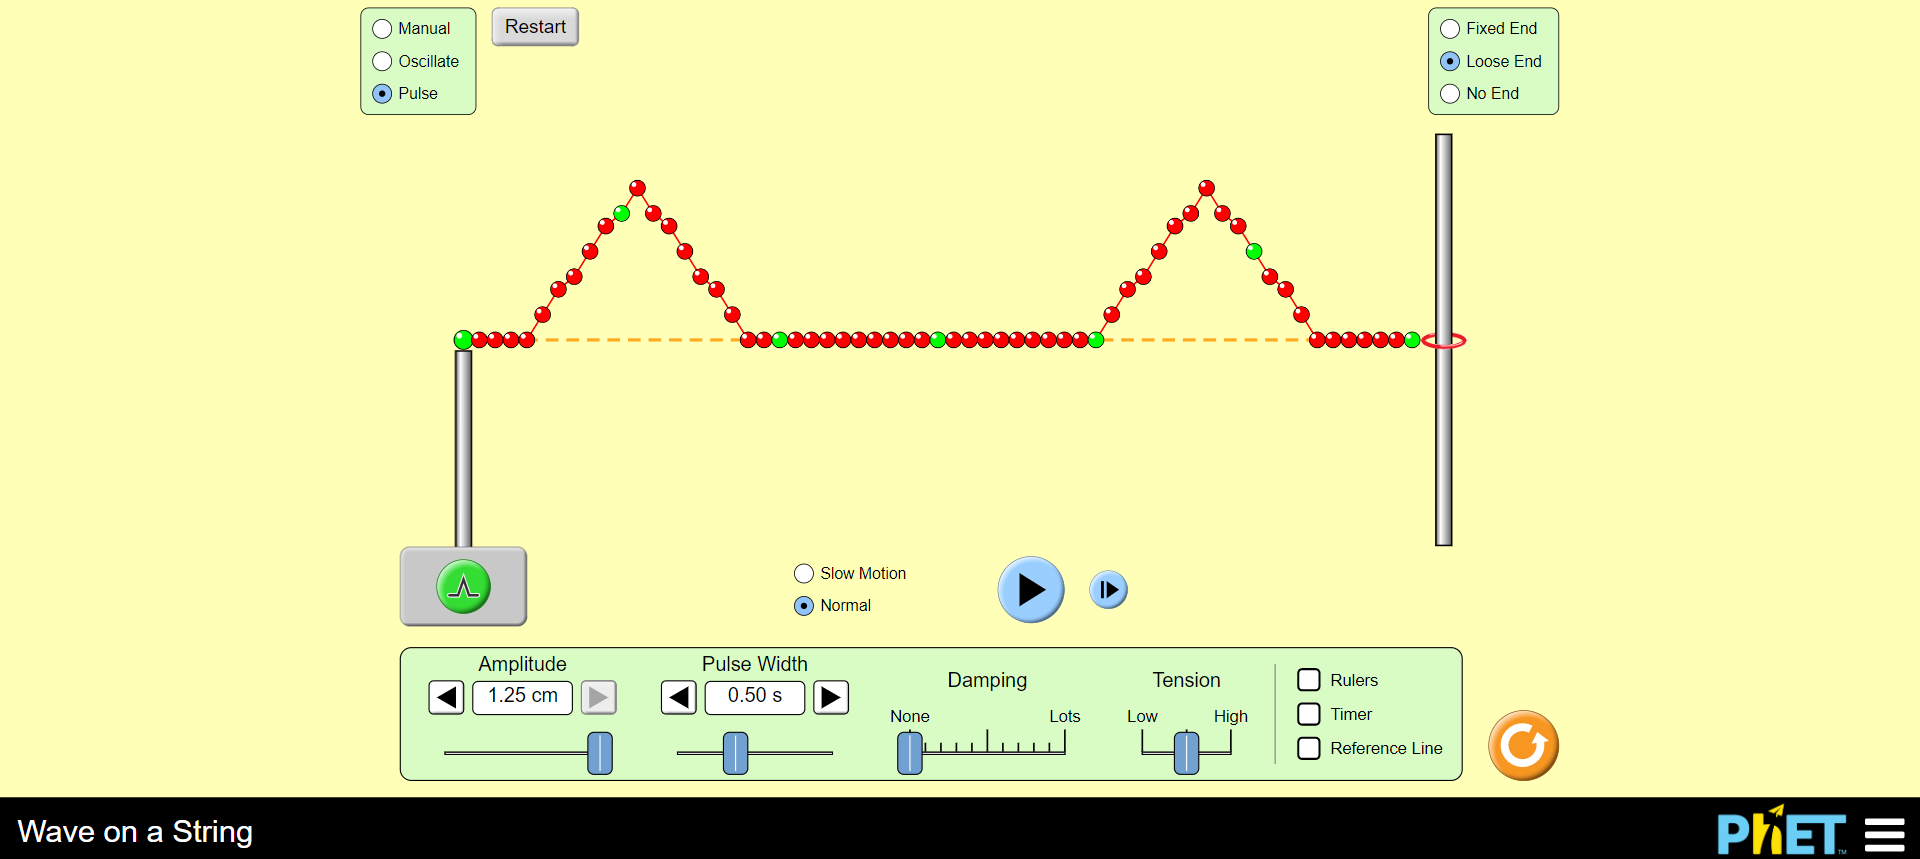
\includegraphics[width=12cm]{physics-2023-24/figures/Unit11_PhET_Wave2.png}
% \end{center}


% \begin{solution}
% When two pulses converge on the same side of the equilibrium line, that portion of the string grows in height as the amplitudes of the two pulses add up. However, when pulses that are on opposite sides converge, the string momentarily flattens as the opposite amplitudes of the pulses cancel each other out.
% \end{solution}



% \begin{multicols*}{2}
% \question
% .

% \begin{tikzpicture}[step=1,x=4mm,y=4mm]
%     \draw[lightgray] (0,0) grid (12,24);
%     \draw[gray] (6,0) -- (6,24);
%     \draw[ultra thick,shift={(0,20)}] (0,0) node[left] {$t = 0$} -- (3,0) -- (3,1) -- (5,1) node[pos=0.5,above] {\large $\rightarrow$} -- (5,0) -- (7,0) -- (7,1) -- (9,1) node[pos=0.5,above] {\large $\leftarrow$} -- (9,0) -- (12,0);
%     \node[left] at (0,4) {$t=4$};
%     \node[left] at (0,8) {$t=3$};
%     \node[left] at (0,12) {$t=2$};
%     \node[left] at (0,16) {$t=1$};
%     \ifprintanswers
%         \draw[red,ultra thick,shift={(0,16)}] (0,0) -- (4,0) -- (4,1) -- (6,1) node[above,pos=0.5] {$\rightarrow$} -- (8,1) node[above,pos=0.5] {$\leftarrow$} -- (8,0) -- (12,0);
%         \draw[red, ultra thick,shift={(0,12)}] (0,0) -- (5,0) -- (5,2) -- (6,2) node[above,pos=0.5] {$\rightarrow$} -- (7,2) node[above,pos=0.5] {$\leftarrow$} -- (7,0) -- (12,0);
%         \draw[red,ultra thick,shift={(0,8)}] (0,0) -- (4,0) -- (4,1) -- (6,1) node[above,pos=0.5] {$\leftarrow$} -- (8,1) node[above,pos=0.5] {$\rightarrow$} -- (8,0) -- (12,0);
%         \draw[red,ultra thick,shift={(0,4)}] (0,0) -- (3,0) -- (3,1) -- (5,1) node[pos=0.5,above] {\large $\leftarrow$} -- (5,0) -- (7,0) -- (7,1) -- (9,1) node[pos=0.5,above] {\large $\rightarrow$} -- (9,0) -- (12,0);
%     \fi
% \end{tikzpicture}

% \question
% .

% \begin{tikzpicture}[step=1,x=4mm,y=4mm]
%     \draw[lightgray] (0,0) grid (12,24);
%     \draw[gray] (6,0) -- (6,24);
%     \draw[ultra thick,shift={(0,20)}] (0,0) node[left] {$t = 0$} -- (3,0) -- (3,1) -- (5,1) node[pos=0.5,above] {\large $\rightarrow$} -- (5,0) -- (6,0) -- (7,0) -- (7,-1) -- (9,-1) node[pos=0.5,below] {\large $\leftarrow$} -- (9,0) -- (12,0);
%     \node[left] at (0,4) {$t=4$};
%     \node[left] at (0,8) {$t=3$};
%     \node[left] at (0,12) {$t=2$};
%     \node[left] at (0,16) {$t=1$};
%     \ifprintanswers
%         \draw[red,ultra thick,shift={(0,16)}] (0,0) -- (4,0) -- (4,1) -- (6,1) node[above,pos=0.5] {$\rightarrow$} -- (6,0) -- (6,-1) -- (8,-1) node[below,pos=0.5] {$\leftarrow$} -- (8,0) -- (12,0);
%         \draw[red, ultra thick,shift={(0,12)}] (0,0) -- (12,0);
%         \draw[red,ultra thick,shift={(0,8)}] (0,0) -- (4,0) -- (4,-1) -- (6,-1) node[below,pos=0.5] {$\leftarrow$} -- (6,0) -- (6,1) -- (8,1) node[above,pos=0.5] {$\rightarrow$} -- (8,0) -- (12,0);
%         \draw[red,ultra thick,shift={(0,4)}] (0,0) -- (3,0) -- (3,-1) -- (5,-1) node[pos=0.5,below] {\large $\leftarrow$} -- (5,0) -- (7,0) -- (7,1) -- (9,1) node[pos=0.5,above] {\large $\rightarrow$} -- (9,0) -- (12,0);
%     \fi
% \end{tikzpicture}

% \vspace*{\fill}

% \columnbreak

% \question
% .

% \begin{tikzpicture}[step=1,x=4mm,y=4mm]
%     \draw[lightgray] (0,0) grid (12,24);
%     \draw[gray] (6,0) -- (6,24);
%     \draw[ultra thick,shift={(0,20)}] (0,0) node[left] {$t = 0$} -- (3,0) -- (3,1) -- (4,1) node[pos=0.5,above] {\large $\rightarrow$} -- (4,-1) -- (5,-1) -- (5,0) -- (6,0) -- (7,0) -- (7,-1) -- (8,-1) -- (8,1) -- (9,1) node[pos=0.5,above] {\large $\leftarrow$} -- (9,0) -- (12,0);
%     \node[left] at (0,4) {$t=4$};
%     \node[left] at (0,8) {$t=3$};
%     \node[left] at (0,12) {$t=2$};
%     \node[left] at (0,16) {$t=1$};
%     \ifprintanswers
%         \draw[red,ultra thick,shift={(0,16)}] (0,0) -- (3,0);
%     \fi
% \end{tikzpicture}

% \question
% .

% \begin{tikzpicture}[step=1,x=4mm,y=4mm]
%     \draw[lightgray] (0,0) grid (12,24);
%     \draw[gray] (6,0) -- (6,24);
%     \draw[ultra thick,shift={(0,20)}] (0,0) node[left] {$t = 0$} -- (3,0) -- (3,1) -- (4,1) node[pos=0.5,above] {\large $\rightarrow$} -- (4,-1) -- (5,-1) -- (5,0) -- (6,0) -- (7,0) -- (7,1) -- (8,1) node[pos=0.5,above] {\large $\leftarrow$} -- (8,-1) -- (9,-1)  -- (9,0) -- (12,0);
%     \node[left] at (0,4) {$t=4$};
%     \node[left] at (0,8) {$t=3$};
%     \node[left] at (0,12) {$t=2$};
%     \node[left] at (0,16) {$t=1$};
%     \ifprintanswers
%         \draw[red,ultra thick,shift={(0,16)}] (0,0) -- (3,0);
%     \fi
% \end{tikzpicture}

% \vspace*{\fill}

% \question
% .

% \begin{tikzpicture}[step=1,x=4mm,y=4mm]
%     \draw[lightgray] (0,0) grid (12,24);
%     \draw[gray] (6,0) -- (6,24);
%     \draw[ultra thick,shift={(0,20)}] (0,0) node[left] {$t = 0$} -- (2,0) -- (2,1) -- (5,1) node[pos=0.5,above] {\large $\rightarrow$} -- (5,0) -- (6,0) -- (7,0) -- (7,-1) -- (8,-1) node[pos=0.5,below] {\large $\leftarrow$} -- (8,0) -- (12,0) ;
%     \node[left] at (0,4) {$t=4$};
%     \node[left] at (0,8) {$t=3$};
%     \node[left] at (0,12) {$t=2$};
%     \node[left] at (0,16) {$t=1$};
%     \ifprintanswers
%         \draw[red,ultra thick,shift={(0,16)}] (0,0) -- (3,0);
%     \fi
% \end{tikzpicture}

% \question
% .

% \begin{tikzpicture}[step=1,x=4mm,y=4mm]
%     \draw[lightgray] (0,0) grid (12,24);
%     \draw[gray] (6,0) -- (6,24);
%     \draw[ultra thick,shift={(0,20)}] (0,0) node[left] {$t = 0$} -- (2,0) -- (2,1) -- (5,1) node[pos=0.5,above] {\large $\rightarrow$} -- (5,0) -- (6,0) -- (7,0) -- (7,1) -- (8,1) node[pos=0.5,above] {\large $\leftarrow$} -- (8,0) -- (12,0) ;
%     \node[left] at (0,4) {$t=4$};
%     \node[left] at (0,8) {$t=3$};
%     \node[left] at (0,12) {$t=2$};
%     \node[left] at (0,16) {$t=1$};
%     \ifprintanswers
%         \draw[red,ultra thick,shift={(0,16)}] (0,0) -- (3,0);
%     \fi
% \end{tikzpicture}

% \end{multicols*}

% \end{questions}

\clearpage



\subsection{Longitudinal Waves}

\begin{questions}
    
\question
Between a compression and a rarefaction, which is below atmospheric pressure?


\question
Name the part of a sound wave that is slightly above atmospheric pressure.


\question
Watch ``How Do Noise Canceling Headphones Work?'' by \texttt{Branch Education} on \texttt{YouTube} (\href{https://youtu.be/VIi04uD8LtY}{click here}). In your own words, briefly summarize how noise-cancelling headphones work. Use the terms defined in this section.


\question \label{J5ZJhe}
Whales emit deep sounds through the ocean. Find Table 14.1 in \texttt{OpenStax: Physics} (\href{https://openstax.org/books/physics/pages/14-1-speed-of-sound-frequency-and-wavelength#Table_14_01}{click here}). What is the speed of a sound wave through sea water? Between air and water, through which medium does sound travel faster?


\question
Access the table from Exercise \ref{J5ZJhe}. Identify the media through which sound waves travel the slowest and the fastest.

\end{questions}



\clearpage
\subsection{Electromagnetic Waves}

\begin{questions}

\question
Which of the following words best answers the question \textit{What is light}?


\begin{center}
    \textbf{
    acceleration \hfill
    charge \hfill
    current \hfill
    energy \hfill
    force \hfill
    momentum \hfill
    position \hfill
    velocity \hfill
    }
\end{center}



\question
Physicists have divided the electromagnetic spectrum into how many different regions?


\question
Name all the regions of the electromagnetic spectrum.


\question
What are some differences between the various types of electromagnetic radiation?


\question
How does wavelength change as frequency \textit{increases} across the electromagnetic spectrum?


\question
Can electromagnetic waves travel through empty space (that is, through a vacuum)?


\question
Create a table with the first column labeled ``visible'' and the second one ``invisible.'' Sort all regions of the electromagnetic spectrum into this table according to whether waves in those regions are visible or invisible to the human eye.



\question
An electromagnetic wave consists of two oscillating fields that are perpendicular and in phase with each other. What are the names of each field?


\question
Generate a radio wave by wiggling an electron. Access the \texttt{PhET Simulation} ``Radio Waves \& Electromagnetic Fields'' (\href{https://phet.colorado.edu/en/simulations/radio-waves}{click here}). Click the play button in the center of the screen. Wiggle the electron, either in \texttt{Manual} or \texttt{Oscillate} mode. Observe how the oscillation of the electric charge results in the propagation in an electromagnetic wave. Use this simulation to explain, in your own words, how all electromagnetic radiation is generated.


\question
The first wave below represents an electromagnetic wave in the X-ray region of the spectrum. If the second wave is not an X-ray, what type of electromagnetic radiation does it represent?


\begin{center}
\begin{tikzpicture}
\begin{axis}[width=16cm,height=3cm,
    xmin=0,xmax=14,
    ymin=-1,ymax=1,
    clip=false,
    ticks=none,
    axis line style={draw=none}
    ]
    \draw[dashed,<->] (0.5,1.05) -- ++(axis direction cs: 2,0);
    \draw plot[domain=0:6*pi, samples=200] (\x/pi,{sin(\x r)});
    \node[above=2mm] at (3,1) {X-ray};
    \begin{scope}[shift={(axis direction cs: 8,0)}]
        \draw plot[domain=0:6*pi, samples=1200] (\x/pi,{sin(7/1*\x r)});
        \draw[dashed,<->] (0.5*1/7,1.05) -- ++(axis direction cs: 2,0);
        \node[above=2mm] at (3,1) {???};    
    \end{scope}
\end{axis}
\end{tikzpicture}
\end{center}

\question
The first wave represents a microwave. If the second wave is an a different region of the spectrum, what type of electromagnetic wave is it?


\begin{center}
\begin{tikzpicture}
\begin{axis}[width=16cm,height=3cm,
    xmin=0,xmax=14,
    ymin=-1,ymax=1,
    clip=false,
    ticks=none,
    axis line style={draw=none}
    ]
    \draw plot[domain=0:6*pi, samples=1200] (\x/pi,{sin(7/1*\x r)});
    \draw[dashed,<->] (0.5*1/7,1.05) -- ++(axis direction cs: 2,0);
    \node[above=2mm] at (3,1) {Microwave};
    \begin{scope}[shift={(axis direction cs: 8,0)}]
        \draw plot[domain=0:6*pi, samples=200] (\x/pi,{sin(\x r)});
        \draw[dashed,<->] (0.5,1.05) -- ++(axis direction cs: 2,0);
        \node[above=2mm] at (3,1) {???};    
    \end{scope}
\end{axis}
\end{tikzpicture}
\end{center}

\question \label{wqaTm6}
When water molecules are bathed in electromagnetic radiation at just the right frequency, they get begin to vibrate and give off heat to their environment. What frequency must these waves have for this phenomenon to occur? Write the number in scientific and decimal notation.


\question
To what region of the electromagnetic spectrum do the waves from Exercise \ref{wqaTm6} belong? 


\question
What happens to the energy of electromagnetic radiation as frequency decreases?


\question
How do humans detect infrared radiation?


\question
Explain some applications of microwaves in astronomy. 


\question
Which type of electromagnetic wave has the longest wavelength of the whole spectrum?


\question
In what medical technology are radio waves used?

\question
Which type of electromagnetic radiation has the shortest wavelengths?


\question
Which form of EM radiation has the most penetrating ability?


\question
Why are high-frequency gamma rays more dangerous to humans than visible light?
\end{questions}


\subsection{Visible Light}

\begin{questions}


\question
Explain Roy G.~Biv.


\question
Identify the name of the cells in your eyes that allow you to perceive color.


\question
What are the seven colors of the rainbow in order of increasing \textit{wavelength}?


\question
Between red and violet, which color represents the high-frequency limit of the visible spectrum?


\question
Which color represents the long-wavelength limit of the visible spectrum?


\question
Which region of the electromagnetic spectrum, apart from visible light, can bees see?


\question
Which animal can see infrared light?


\question \label{lwLSKO}
Sort the colors yellow, blue, and red from shortest wavelength to longest.



\question
Convert \SI{5798}{nm} to meters, writing in scientific notation.


\question
Sort the colors in Exercises \ref{lwLSKO} from lowest frequency to highest.


\question
What is the wavelength of a red light wave that has a frequency of \SI{4.746e14}{\Hz} if the wave travels through empty space at a speed of \SI{3.0e8}{m/s}? Express your answer in nanometers (nm).


\question
The Bacillus is a species of rod-shaped bacteria that are very common in nature. As shown below, a typical length is about 2 to 6 microns. Consider a green light wave, which has a wavelength of about 500 nanometers. About how many wave cycles of green light could fit along the length of the Bacillus below?



\begin{center}
\begin{tikzpicture}
\begin{axis}[width=16cm,height=2.5cm,
    xmin=0,xmax=12,
    ymin=-1,ymax=1,
    clip=false,
    ticks=none,
    axis line style={draw=none}
    ]
    \draw plot[domain=0:4*pi, samples=1200] (\x/pi,{sin(7/1*\x r)});
    \begin{scope}[shift={(axis direction cs: 8,0)}]
        \draw plot[domain=0:4*pi, samples=200] (\x/pi,{sin(\x r)});   
    \end{scope}
\end{axis}
\end{tikzpicture}

\vspace{-1.5cm}

\begin{tikzpicture}
    \draw[fill=lightgray] (0,0) circle (0.5);
    \begin{scope}[shift={(2,0)}]
        \draw[fill=lightgray] (0,0) circle (0.5); 
    \end{scope}
    \fill[lightgray] (0,-0.5) rectangle ++(2,1) node[black,pos=0.5] {\textbf{bacillus}};
    \draw (0,0.5) -- ++(2,0)
          (0,-0.5) -- ++(2,0);
    \draw[<->] (-0.5,0.7) -- ++(3,0) node[above,pos=0.5] {\SI{5}{\micro\meter}};
\end{tikzpicture}
\end{center}


\question
True or false? Light requires a medium to propagate.


\question
What is the value of $c$, the speed of light in a vacuum?


\question
Saturn is \SI{1.43e12}{m} from the Sun. How many minutes does it take the Sun’s light to reach Saturn? To get full credit, show all your work.
\end{questions}

\subsection{Optics}

{\large \textbf{Other}}

\begin{questions}
    
\question
The first wave below represents the electromagnetic wave for the color cyan, which is indicated in the visible spectrum below. The dashed double arrows are the same length. Which color could be represented by the second wave?

\begin{center}
\begin{tikzpicture}
\begin{axis}[width=16cm,height=3cm,
    xmin=0,xmax=24,
    ymin=-1,ymax=1,
    clip=false,
    ticks=none,
    axis line style={draw=none}
    ]
    \draw[dashed,<->] (0.5,1.05) -- ++(axis direction cs: 2,0);
    \draw plot[domain=0:10*pi, samples=200] (\x/pi,{sin(\x r)});
    \node[above=2mm] at (4.5,1) {cyan};
    \begin{scope}[shift={(axis direction cs: 12,0)}]
        \draw[dashed,<->] (0.5*632/490,1.05) -- ++(axis direction cs: 2,0);
        \draw plot[domain=0:10*pi, samples=500] (\x/pi,{sin(490/632*\x r)});
        \node[above=2mm] at (5,1) {???};    
    \end{scope}
\end{axis}
\end{tikzpicture}

\vspace{1em}

\begin{tikzpicture}
    \begin{axis}[width=14cm, height=7cm,
        ymin=0,ymax=1,
        height=3cm,
        xmin=360,xmax=740,
        yticklabels={},
        ytick=\empty,
        axis lines=left,
        separate axis lines,
        y axis line style=white,
        x dir=reverse,
        clip=false,
        ticks=none,
        axis line style={draw=none}
        ]
        \addplot[draw=none, name path=uv, forget plot] coordinates{(360,0)(360,0.5)};
        \addplot[draw=none, name path=visible, forget plot] coordinates{(740,0)(740,0.5)};
        \addplot[shading=visiblelight, area legend] fill between[of=uv and visible];
        \draw[<-,thick] (490,0.5) -- ++(axis direction cs: 0,0.4) node[above] {cyan};
    \end{axis}
\end{tikzpicture}
\end{center}

\begin{randomizechoices}
    \correctchoice red
    \choice violet
    \choice indigo
    \choice ultraviolet 
\end{randomizechoices}

\question 
The first wave represents a green electromagnetic wave. The second wave is an electromagnetic wave that is invisible to the human eye. Assume the double dashed arrows are the same size. What type of electromagnetic wave could be represented by the second wave?

\begin{center}
\begin{tikzpicture}
\begin{axis}[width=16cm,height=3cm,
    xmin=0,xmax=24,
    ymin=-1,ymax=1,
    clip=false,
    ticks=none,
    axis line style={draw=none}
    ]
    \draw[dashed,<->] (0.5,1.05) -- ++(axis direction cs: 2,0);
    \draw plot[domain=0:10*pi, samples=200] (\x/pi,{sin(\x r)});
    \node[above=2mm] at (4.5,1) {green};
    \begin{scope}[shift={(axis direction cs: 12,0)}]
        \draw[dashed,<->] (0.5*200/550,1.05) -- ++(axis direction cs: 2,0);
        \draw plot[domain=0:10*pi, samples=500] (\x/pi,{sin(550/200*\x r)});
        \node[above=2mm] at (5,1) {???};    
    \end{scope}
\end{axis}
\end{tikzpicture}
\end{center}

\begin{randomizechoices}
    \correctchoice ultraviolet
    \choice microwave
    \choice blue light
    \choice gamma ray
    \choice radio wave
\end{randomizechoices}


\question
The diagram below represents a transverse wave.

\def\twopi{2*pi}

\begin{tikzpicture}
\begin{axis}[width=8cm,height=4cm,
        axis lines=center,
        clip=false,
        ticks=none,
        axis line style={draw=none},
]
\addplot [thick,
    domain=0:1.5*\twopi, 
    samples=200, 
    color=black,
]
{sin(deg(x))};
    \draw[black!50] (-1,0) -- ++(axis direction cs: 3*pi+2,0);
    \fill (0,0) circle (2pt) node[below] {A};
    \fill (pi/2,1) circle (2pt) node[above] {B};
    \fill (pi,0) circle (2pt) node[below left] {C};
    \fill (3*pi/2,-1) circle (2pt) node[below] {D};
    \fill (2*pi,0) circle (2pt) node[above left] {E};
    \fill (5*pi/2,1) circle (2pt) node[below] {F};
    \fill (3*pi,0) circle (2pt) node[below] {G};

\end{axis}
\end{tikzpicture}

The wavelength of the wave is equal to the distance between points \fillin .

\begin{randomizechoices}
    \correctchoice B and F
    \choice A and G
    \choice D and F
    \choice C and E
\end{randomizechoices}

\question
 The energy of a sound wave is most closely related to its \fillin\ .

 \begin{randomizechoices}
     \correctchoice amplitude
     \choice wavelength
     \choice frequency
     \choice period
\end{randomizechoices}

\question
The diagram below represents a transverse wave.

\begin{tikzpicture}
\begin{axis}[width=8cm,height=4cm,
    ticks=none,
    clip=false,
    axis lines=center,
]

\addplot[
    domain=pi:3*pi,
    samples=100,
    color=black,
]
{sin(deg(x))};
    \fill (pi,1) circle (2pt) node[left] {D};
    \fill (pi,0) circle (2pt) node[left] {A};
    \fill (pi,-1) circle (2pt) node[left] {E};
    
\end{axis}
\end{tikzpicture}




\question %27
Describe the electric and magnetic fields that make up an electromagnetic wave.

\begin{center}
    \centering
    \scalebox{0.9}{
    \begin{tikzpicture}[x={(-10:1cm)},y={(90:1cm)},z={(210:1cm)}]
    % Axes
    \draw (-1,0,0) node[above] {$x$} -- (5,0,0);
    \draw (0,0,0) -- (0,2,0) node[above] {$y$};
    \draw (0,0,0) -- (0,0,2) node[left] {$z$};
    % Propagation
    \draw[->,ultra thick] (5,0,0) -- node[above] {$c$} (6,0,0);
    % Waves
    \draw[blue,thick] plot[domain=0:4.5,samples=200] (\x,{cos(deg(pi*\x))},0);
    \draw[red,thick] plot[domain=0:4.5,samples=200] (\x,0,{cos(deg(pi*\x))});
    % Arrows
    \foreach \x in {0.1,0.3,...,4.4} {
      \draw[->,help lines] (\x,0,0) -- (\x,{cos(deg(pi*\x))},0);
      \draw[->,help lines] (\x,0,0) -- (\x,0,{cos(deg(pi*\x))});
    }
    % Labels
    \node[above right] at (0,1,0) {$\boldsymbol{E}$};
    \node[below] at (0,0,1) {$\boldsymbol{B}$};
    \end{tikzpicture}
    }
\end{center}

\begin{choices}
\choice They are perpendicular to and out of phase with each other.
\CorrectChoice They are perpendicular to and in phase with each other.
\choice They are parallel to and out of phase with each other.
\choice They are parallel to and in phase with each other.
\end{choices}

% \begin{solution}
% They are at right angles (OR \ang{90} OR perpendicular) to each other and they are in phase.
% \end{solution}

\question
What are the 7 regions of the electromagnetic spectrum?


\begin{choices}
\choice infrared, hertz, joule, kilogram, energy, visible light, ultraviolet
\choice gamma ray, microwave, mass, velocity, energy, speed, X-ray
\choice newton, hertz, joule, velocity, energy, speed, X-ray
\correctchoice radio, microwave, infrared, visible, ultraviolet, X-ray, gamma ray
\end{choices}

\question
How does wavelength change as frequency \textit{increases} across the electromagnetic spectrum?


\begin{choices}
\choice Wavelength increases.
\choice Wavelength first increases and then decreases.
\choice Wavelength first decreases and then increases.
\CorrectChoice Wavelength decreases.
\end{choices}

\question
Which portion of the electromagnetic spectrum is \textit{not invisible} to the human eye?

\begin{choices}
\choice microwave
\choice infrared
\CorrectChoice visible light
\choice x-ray
\end{choices}

\question
What are the 7 colors of visible light?

\begin{choices}
\choice magenta, cyan, yellow, green, brown, black, white
\correctchoice red, orange, yellow, green, blue, indigo, violet
\choice magenta, cyan, yellow, green, red, orange, white
\choice red, orange, yellow, green, brown, cyan, pink
\end{choices}

\question
If the first wave is green light, which color could be represented by the second wave?

\begin{center}
    \centering
    \begin{tikzpicture}
        \draw[thick] plot[domain=0:3*2*pi, samples=500]  (\x/pi,{0.8*sin(\x r)});
        \node at (3,1.2) {GREEN LIGHT WAVE};
        \draw[thick] plot[domain=3.5*2*pi:6.5*2*pi, samples=500]  (\x/pi,{0.8*sin(3*\x r)});
        \node at (10,1.2) {???};
    \end{tikzpicture}
\end{center}

\begin{choices}
\choice red
\choice yellow
\correctchoice blue
\choice infrared
\end{choices}



\clearpage


\question
In addition to visible light, bees can also see the \fillin\ region of the electromagnetic spectrum. 

\begin{choices}
\correctchoice ultraviolet
\choice infrared
\choice radio
\choice X-ray
\end{choices}


\question % 2
Consider these colors of light: 

\begin{center}
    \textbf{yellow, blue, red}
\end{center}


Put these light waves in order according to \textit{wavelength}, from shortest wavelength to longest wavelength.

\begin{choices}
\choice blue, yellow, red
\choice red, yellow, blue
\choice red, yellow, blue
\CorrectChoice blue, yellow, red
\end{choices}

% \begin{solution}
% Blue has the shortest wavelength and the highest frequency of the colors given while red has the longest wavelength and the smallest frequency.
% \end{solution}

\question % 2
Consider these colors of light: 

\begin{center}
    \textbf{yellow, blue, red}
\end{center}

Put these light waves in order according to \textit{frequency}, from lowest frequency to highest frequency.

\begin{choices}
\choice blue, yellow, red
\choice red, yellow, blue
\choice blue, yellow, red
\CorrectChoice red, yellow, blue
\end{choices}

\question
Red light has a wavelength of \SI{700}{nm}. Assuming red light moves at the speed of light in a vacuum, at \SI{3.0e8}{m/s}, what is the frequency of red light?

\begin{choices}
\choice \SI{2.3e-15}{Hz}
\choice \SI{210}{Hz}
\correctchoice \SI{4.3e14}{Hz}
\choice \SI{4.76e-4}{Hz}
\end{choices}

\question
Violet light has a wavelength of \SI{400}{nm}. Assuming violet light moves at the speed of light in a vacuum, at \SI{3.0e8}{m/s}, what is the frequency of violet light?

\begin{choices}
\choice \SI{2.3e-15}{Hz}
\choice \SI{210}{Hz}
\correctchoice \SI{7.5e14}{Hz}
\choice \SI{4.76e-4}{Hz}
\end{choices}

\clearpage
\question 
The first wave represents red light. Which EM wave could be represented by the other wave?

\begin{center}
    \centering
    \begin{tikzpicture}
        \draw[thick] plot[domain=0:3*2*pi, samples=500]  (\x/pi,{0.8*sin(3*\x r)});
        \node at (10,1.2) {???};
        \draw[thick] plot[domain=3.5*2*pi:6.5*2*pi, samples=500]  (\x/pi,{0.8*sin(\x r)});
        \node at (3,1.2) {RED LIGHT WAVE};
    \end{tikzpicture}
\end{center}

\begin{choices}
\choice green light
\choice ultraviolet
\choice X-ray
\correctchoice infrared
\end{choices}

\question % 4
In which region of the electromagnetic spectrum would you find radiation that is invisible to the human eye and has low energy?

\begin{choices}
\choice Long-wavelength and high-frequency region
\CorrectChoice Long-wavelength and low-frequency region
\choice Short-wavelength and high-frequency region
\choice Short-wavelength and low-frequency region
\end{choices}

\question
Which scientist discovered infrared light?

\begin{choices}
\choice Albert Einstein (1905)
\choice Isaac Newton (1661)
\correctchoice William Herschel (1800)
\choice Madam Curie (1903)
\end{choices}

\question %26
Describe one way in which heat waves---infrared radiation---are different from sound waves.

\begin{choices}
\choice Sound waves are transverse waves, whereas heat waves---infrared radiation---are longitudinal waves.
\choice Sound waves have shorter wavelengths than heat waves.
\CorrectChoice Sound waves require a medium, whereas heat waves---infrared radiation---do not.
\choice Sound waves have higher frequencies than heat waves.
\end{choices}

% \begin{solution}
% Heat waves can travel across empty space and sound waves cannot.
% \end{solution}

\vspace{1em}
\hrule 

\clearpage
\begin{EnvUplevel}
\textbf{Read the prompt below. Then answer questions \ref{ques:fire_first} through \ref{ques:fire_last}.}

When you stand in front of an open fire, you can sense light waves with your eyes. You sense another type of electromagnetic radiation as heat.
\end{EnvUplevel}


\question \label{ques:fire_first} %8
How are the light waves and heat waves radiated by the fire the same, and how are they different?

\begin{choices}
\choice Both travel as waves, but only light waves are a form of electromagnetic radiation.
\CorrectChoice Heat and light are both forms of electromagnetic radiation, but light waves have higher frequencies.
\choice Heat and light are both forms of electromagnetic radiation, but heat waves have higher frequencies.
\choice Heat and light are both forms of electromagnetic radiation, but light waves have higher wavelengths.
\end{choices}

% \begin{solution}
% Heat and light waves are both forms of electromagnetic radiation, but they have different frequencies. Our eyes detect only the range of frequencies called visible light. The heat waves are easily absorbed by our body, but the light is mostly reflected.
% \end{solution}

\question %10
What is this other type of radiation?

\begin{choices}
\choice Visible light rays
\choice X-rays
\choice Gamma rays
\CorrectChoice Infrared rays
\end{choices}


\question \label{ques:fire_last} %10
How is this other type of radiation different from light waves?

\begin{choices}
\choice The visible light rays have higher frequencies and shorter wavelengths than the light waves.
\CorrectChoice The infrared rays have lower frequencies and longer wavelengths than the light waves.
\choice The X-rays have lower frequencies and longer wavelengths than the light waves.
\choice The gamma rays have higher frequencies and shorter wavelengths than the light waves.
\end{choices}
\vspace{1em}

\hrule

% \begin{solution}
% Part A. We sense infrared waves as heat. Part B. We sense the light with our eyes and the heat with our whole body. The heat waves have lower frequency and longer wavelengths than the light waves. They are both forms of electromagnetic radiation.
% \end{solution}

\question
What is the value of $c$, the speed of light in a vacuum?

\begin{choices}
\correctchoice \SI{3.0e8}{m/s} (3 million meters per second)
\choice \SI{0.0}{m/s} (zero meters per second)
\choice \SI{1.0e5}{m/s} (100 thousand meters per second)
\choice \SI{584}{m/s} (584 meters per second)
\end{choices}

\question
When light travels through a physical medium, its speed is always \fillin[][0.8in]\ the speed of light ($c$).

\begin{choices}
\choice greater than
\choice equal to
\choice negative
\correctchoice less than
\end{choices}

\question
Light travels in water at \fillin\ the value of $c$.

\begin{choices}
\correctchoice $3/4$
\choice $1/2$
\choice $5/6$
\choice $2/3$
\end{choices}

\question
In air, light has a speed that is \fillin\ of $c$.

\begin{choices}
\choice 0.03 percent
\choice 65.00 percent
\correctchoice 99.97 percent
\choice 87.50 percent
\end{choices}

\question
Diamond slows light down to just \fillin\ of $c$.

\begin{choices}
\correctchoice 41 percent
\choice 33 percent
\choice 61 percent
\choice 74 percent
\end{choices}

\question %5
Light travels at different speeds in different media. Put these media in order, from the slowest light speed to the fastest light speed: air, diamond, vacuum, water.

\begin{choices}
\choice vacuum, diamond, air, water
\choice diamond, air, water, vacuum
\correctchoice diamond, water, air, vacuum
\choice air, diamond, water, vacuum
\end{choices}

\question %28
Explain how X-ray radiation can be harmful and how can it be a useful diagnostic tool.

\begin{choices}
\choice Overexposure to X-rays can cause HIV, though normal levels of X-rays can be used for sterilizing needles.
\CorrectChoice Overexposure to X-rays can cause cancer, though in limited doses X-rays can be used for imaging internal body parts.
\choice Overexposure to X-rays causes diabetes, though normal levels of X-rays can be used for imaging internal body parts.
\choice Overexposure to X-rays causes cancer, though normal levels of X-rays can be used for reducing cholesterol in the blood.
\end{choices}

\question %17
Which type of electromagnetic radiation has the shortest wavelengths?

\begin{choices}
\CorrectChoice Gamma rays
\choice Infrared waves
\choice Blue light
\choice Microwaves
\end{choices}

\question %18
Which form of EM radiation has the most penetrating ability?

\begin{choices}
\choice red light
\choice microwaves
\choice gamma rays
\choice infrared radiation
\end{choices}


\question % 3
What is the location of gamma rays on the electromagnetic spectrum?

\begin{choices}
\choice At the high-frequency and long-wavelength end of the spectrum
\CorrectChoice At the high-frequency and short-wavelength end of the spectrum
\choice At the low-frequency and long-wavelength end of the spectrum
\choice At the low-frequency and short-wavelength end of the spectrum
\end{choices}

\question %19
Why are high-frequency gamma rays more dangerous to humans than visible light?

\begin{choices}
\choice Gamma rays have a lower frequency range than visible light.
\choice Gamma rays have a longer wavelength range than visible light.
\CorrectChoice Gamma rays have greater energy than visible light for penetrating matter.
\choice Gamma rays have less energy than visible light for penetrating matter.
\end{choices}



\question %33
Saturn is \SI{1.43e12}{m} from the Sun. How many minutes does it take the Sun’s light to reach Saturn?

\begin{choices}
\choice \SI{7.94e9}{min}
\choice \SI{3.4e4}{min}
\choice \SI{3.4e-6}{min}
\choice \SI{79.4}{min}
\end{choices}


\question %34
A frequency of red light has a wavelength of \SI{700}{nm}. Violet light has a \fillin[higher] frequency and \fillin[shorter] wavelength than red light.

\vspace{0.5em}

\begin{choices}
\choice lower; longer
\CorrectChoice higher; shorter
\choice lower; shorter
\choice higher; longer
\end{choices}

% \begin{solution}
% Violet light has a higher frequency and shorter wavelength than red light.
% \end{solution}


\question %34
A frequency of red light has a wavelength of \SI{700}{nm}. Which type of radiation has lower frequencies than red light?

\vspace{0.5em}

\begin{choices}
\choice ultraviolet radiation
\choice x-ray radiation
\CorrectChoice infrared radiation
\choice violet light radiation

\end{choices}

% \begin{solution}
% Infrared radiation or any other type of radiation in the low-frequency end of the spectrum.
% \end{solution}

\question %34
A frequency of red light has a wavelength of \SI{700}{nm}. Which type of radiation has shorter wavelengths than violet light?

\vspace{0.5em}

\begin{choices}
\choice infrared radiation
\CorrectChoice ultraviolet radiation
\choice red light radiation
\choice microwave radiation
\end{choices}

% \begin{solution}
% Ultraviolet radiation or any other type of radiation in the high-frequency end of the spectrum.
% \end{solution}

\question %22
What is the wavelength of red light with a frequency of \SI{4.00e14}{\Hz}?

\begin{choices}
\choice \SI{2.50e14}{\meter}
\choice \SI{4.00e15}{\meter}
\choice \SI{2.50e6}{\meter}
\CorrectChoice \SI{7.50e-7}{\meter}
\end{choices}

\begin{solution}
The \textit{Known} quantities:

\begin{itemize}
    \item frequency: $f = \SI{4.00e14}{\Hz}$
    \item speed of light: $c = \SI[per-mode=symbol]{3.00e8}{\meter\per\second}$
\end{itemize}

Frequency and wavelength are related to the speed of light by

\begin{equation*}
    c = f \lambda
\end{equation*}

Solving for wavelength,

\begin{equation*}
    \lambda = \frac{c}{f} = \SI{7.50e-7}{\meter}
\end{equation*}
\end{solution}

\question %14
Visible light has a range of wavelengths from about \SI{400}{nm} to \SI{800}{nm}. What is the range of frequencies for visible light?

\begin{choices}
\choice \SI{3.75e6}{\Hz} to \SI{7.50e6}{\Hz}
\choice \SI{3.75}{\Hz} to \SI{7.50}{\Hz}
\choice \SI{3.75e-7}{\Hz} to \SI{7.50e-7}{\Hz}
\CorrectChoice \SI{3.75e14}{\Hz} to \SI{7.50e14}{\Hz}
\end{choices}

\begin{solution}
The \textit{Known} quantities:

\begin{itemize}
    \item red limit of wavelength $\lambda_R = \SI{800}{\nano\meter} = \SI{800e-9}{\meter}$
    \item violet limit of wavelength: $\lambda_V = \SI{400}{\nano\meter} = \SI{400e-9}{\meter}$
    \item speed of light: $c = \SI{3.00e8}{\meter/\second}$
\end{itemize}

Frequency and wavelength are related to the speed of light by

\begin{equation*}
    c = f \lambda
\end{equation*}

Solving for frequency,

\begin{equation*}
    f = \frac{c}{\lambda}
\end{equation*}

The red and violet limits of frequency are

\begin{align*}
    f_R = \frac{c}{\lambda_R} = \SI{3.75e14}{\Hz}\\
    \\
    f_V = \frac{c}{\lambda_V} = \SI{7.50e14}{\Hz}\\
\end{align*}
\end{solution}

\end{questions}







